\documentclass[11pt]{article}

\def\PublicationUsePalatino{}
\def\PublicationReadableType{}
\def\PublicationWideMargins{}
\def\PublicationTwoRules{}
\def\PublicationDedicatedFrontPage{}

\usepackage{PRIMEarxiv}

\usepackage[utf8]{inputenc} % allow utf-8 input
\usepackage[T1]{fontenc}    % use 8-bit T1 fonts
\usepackage{hyperref}       % hyperlinks
\usepackage{url}            % simple URL typesetting
\usepackage{booktabs}       % professional-quality tables
\usepackage{amsfonts}       % blackboard math symbols
\usepackage{nicefrac}       % compact symbols for 1/2, etc.
\usepackage{microtype}      % microtypography
\usepackage{lipsum}
\usepackage{fancyhdr}       % header
\usepackage{graphicx}       % graphics
\usepackage{amsmath}        % for math environments like align*
\usepackage{amssymb}        % for math symbols like \mathbb
\usepackage{placeins}
\usepackage{float}          % improved float placement control (H)
\usepackage[capitalize,nameinlink]{cleveref} % better cross-references
\usepackage{algorithm}
\usepackage{algpseudocode}
\usepackage{amsthm}
\usepackage{xcolor}
\usepackage{unified-publication}

\newtheorem{proposition}{Proposition}
\renewcommand{\theproposition}{M\arabic{proposition}}

\theoremstyle{definition}

% Callouts: no heading inside (caller provides any label), comfortable padding
\definecolor{calloutbg}{gray}{0.90}
\newlength{\calloutpad}
\setlength{\calloutpad}{1.0em} % horizontal padding
\ifdefined\HCode
\newcommand{\callout}[1]{%
  \ifvmode\IgnorePar\fi\EndP
  \HCode{<aside class="callout">}%
  #1%
  \ifvmode\IgnorePar\fi\EndP
  \HCode{</aside>}\ShowPar
}
\else
\newcommand{\callout}[1]{%
  \vspace{0.9em}%
  \noindent\colorbox{calloutbg}{%
    \parbox{\dimexpr\linewidth-2\fboxsep\relax}{%
      \hspace*{\calloutpad}%
      \begin{minipage}{\dimexpr\linewidth-2\fboxsep-2\calloutpad\relax}
      \vspace{0.8em}%
      #1\par
      \vspace{0.8em}%
      \end{minipage}%
      \hspace*{\calloutpad}%
    }%
  }%
  \vspace{0.9em}%
}
\fi

\graphicspath{{media/}}     % organize your images and other figures under media/ folder

%Header
\pagestyle{fancy}
\thispagestyle{empty}
\rhead{ \textit{ }} 

% Update your Headers here
\fancyhead[LO]{Temporal Regularized Learning}
% \fancyhead[RE]{Firstauthor and Secondauthor} % Firstauthor et al. if more than 2 - must use \documentclass[twoside]{article}


  
%% Title
\title{Temporal Regularized Learning: Self-supervised learning local in space and time
%%%% Cite as
%%%% Update your official citation here when published 
% \thanks{\textit{\underline{Citation}}: 
% \textbf{Authors. Title. Pages.... DOI:000000/11111.}} 
}

\author{
  Davide R. Wiest \\
  Darmstadt\\
  \texttt{dw@axym.org} \\
}

\publicationtitle{Temporal Regularized Learning: Self-supervised learning local in space and time}
\publicationauthors{Davide R. Wiest}
\publicationaffiliations{Axym Labs, Darmstadt, Germany}
\publicationdate{}

\providecommand{\LeadFigurePath}{figures/terel-lead.pdf}
\providecommand{\LeadFigureMaxHeight}{0.26\textheight}
\providecommand{\LeadFigureCaption}{%
\textbf{Left:} Laplacian-eigenmap projection of TeReL validation
representations, colored by MNIST class. \textbf{Right:} validation accuracy
for the $4\times2000$ setting. TeReL closes the gap to backpropagation to
0.13 percentage points at this scale; Forward-Forward remains the strongest
reported comparison. TeReL, TeReL-S, and BP average five runs, whereas FF is a
reported comparison without matched uncertainty.}


\begin{document}

\begin{publicationhead}
\makepublicationtitle
\publicationleadfigure[\LeadFigureMaxHeight]{\LeadFigurePath}{\LeadFigureCaption}
\publicationabstract{We introduce Temporal Regularized Learning (TeReL), a spatially and temporally local learning rule for self-supervised representation learning from sequential input streams. The key idea is to instantiate a VICReg-style objective with temporally adjacent positives and non-differentiated running population statistics, yielding a per-neuron online loss with bounded state. We also analyze how this perspective connects modern SSL objectives to classical temporal representation learning rules such as Slow Feature Analysis and trace learning.
We present TeReL and a simplified variant, TeReL-S, and evaluate them on MNIST under controlled temporal orderings. Our method achieves competitive accuracy compared to backpropagation, Forward-Forward, and Equilibrium Propagation, while learning highly class-separable representations with rich first-layer receptive fields; TeReL-S attains similar performance despite its more restricted design. We further study a scoped recurrent setting on MNIST-Rows next-row prediction, comparing against a backpropagation-through-time baseline, and provide quantitative latent-trajectories.}
\publicationlinks{%
  \textbf{Code:}\enspace
  \href{https://github.com/Axym-Labs/TeReL}{\nolinkurl{https://github.com/Axym-Labs/TeReL}}\\
  \textbf{Project page:}\enspace
  \href{https://axym.org/work/terel}{\nolinkurl{https://axym.org/work/terel}}\\
  \textbf{Correspondence:}\enspace
  \href{mailto:dw@axym.org}{\nolinkurl{dw@axym.org}}%
}
\publicationhtmlinsertion
\end{publicationhead}

\ifdefined\HCode
  \ifvmode\IgnorePar\fi\EndP
  \HCode{<main id="article-content">}\ShowPar
\fi

\ifdefined\PublicationDedicatedFrontPage
  \clearpage
\fi

\section{Introduction}

Learning from unlabeled sensory streams is a practical necessity for both biological modeling and energy-efficient machine learning on constrained hardware. Modern self-supervised methods succeed on unlabeled data by aligning representations of related samples (positives) while avoiding collapse using either negative samples or explicit regularizers. Contrastive methods rely on negatives and on large batch sizes to estimate cross-sample statistics. \cite{chen2020, oord2018}

Regularized alternatives avoid explicit negatives and instead combine an invariance term with variance and covariance penalties. \cite{bardes2022, zbontar2021, chenhe2021, grill2020} VICReg is a regularized method that enforces invariance without negatives and whose regularizers can be computed from local moments, at least in a batched implementation. \cite{bardes2022}

This paper shows how a VICReg-style objective can be instantiated as a per-neuron temporal loss by using adjacent observations as positives and treating running population statistics as non-differentiated state. The motivation is practical: locality reduces communication between units, and temporal locality permits streaming implementations with only a small short-term memory per neuron. Both properties are desirable for analog and neuromorphic hardware. \cite{indiveri2015, davies2018}

By making the invariance temporal, TeReL is a type of Slow Feature Analysis (SFA) procedure: SFA aims to extract slowly changing features from a temporal sequence of faster-changing inputs. \cite{wiskott2002, foldiak1991} This can lead to representations that are invariant to augmentations or capture latent variables. More broadly, many sequential domains contain latent factors that evolve more slowly than their raw observations. In text, the sentiment of a review remains stable across its many words; in finance, stock prices fluctuate faster than the market factors that drive them; in physiology, the underlying state or health condition of a patient evolves slowly relative to heartbeat, respiratory cycles, and momentary noise in sensor traces.

\paragraph{Contributions}
This paper makes three contributions. First, it derives TeReL from VICReg through an explicit instantiation choice: population statistics are maintained as non-differentiated state, while adjacent observations supply the positive pairs. Second, it clarifies TeReL as a conceptual bridge between modern regularized self-supervised learning objectives and classical temporal representation learning ideas such as Slow Feature Analysis and trace learning, motivating directions for improving existing biologically inspired rules. \cite{foldiak1991, oja1982} Third, it evaluates TeReL and TeReL-S on MNIST with controlled temporal orderings, provides representation diagnostics, and reports a set of diverse ablations. \cite{raghu2017, kornblith2019} In addition, we provide practical hyperparameter guidance based on ablations (Appendix~\ref{app:hyperparam-guidance}); full reproducibility details appear in the appendix.

\paragraph{Paper structure}
Section~\ref{sec:method} derives TeReL from VICReg and reformulates the objective into per-neuron, temporally local loss terms, then discusses memory requirements, simplified gradients, and parallelizability. Section \ref{sec:related} compares this approach to existing work and discusses the relation to Slow Feature Analysis and trace learning. Section~\ref{sec:mnist} evaluates TeReL and TeReL-S on MNIST with controlled temporal orderings, compares against baseline learning rules, and provides representation diagnostics. Section~\ref{sec:mnist_rows_rnn} studies a scoped recurrent setting (MNIST-Rows next-row prediction) under a locality constraint; implementation details needed for reproduction are provided in the appendix.

\section{Method}\label{sec:method}

% NOTE: The duplicate label \label{sec:experiments} was removed (it conflicted with later references).

\callout{\textbf{TL;DR} TeReL is a temporally local, per-neuron learning rule built from three terms: \textbf{temporal coherence}, \textbf{variance}, and \textbf{decorrelation}. Temporal coherence uses time-adjacent samples as positives, variance is maintained by per-neuron running statistics, and decorrelation is enforced by an auxiliary \emph{lateral mapping}. TeReL avoids negative samples and does not backpropagate gradients to earlier layers.}

\subsection{Locality claim and design overview}\label{sec:locality-claim}
\paragraph{Locality definition.}
We call a learning rule \emph{spatially local} if the update of a weight depends only on quantities available at its pre- and postsynaptic units (and optional same-layer auxiliary units) and does not require backpropagated error signals from other layers. We call it \emph{temporally local} (online) if the update at time step $i$ depends only on the current activities and a bounded amount of per-unit state carried forward in time.

\callout{
\begin{proposition}[A stop-gradient population-statistic VICReg instantiation is temporally local]\label{thm:vicreg-local}
Assume an input stream with temporal coherence such that sequentially adjacent
samples can be treated as positive pairs. Instantiate the VICReg decomposition
\begin{equation}
    L_{\mathrm{VIC}} = \lambda_{\mathrm{sim}} L_{\mathrm{sim}}^{\mathrm{rep}} + \lambda_{\mathrm{var}} L_{\mathrm{var}}^{\mathrm{rep}} + \lambda_{\mathrm{cov}} L_{\mathrm{cov}}^{\mathrm{rep}},
\end{equation}
as a weighted sum of temporal coherence, variance, and decorrelation terms,
\begin{equation}
L = \lambda_{S} L_{S} + \lambda_{V} L_{V} + \lambda_{C} L_{C}.
\end{equation}
where running means and variances are treated as state and are not
differentiated through their update histories. If the decorrelation term is
supplied by a detached same-layer lateral mapping, the gradient at time $t$
depends only on the current activation, the preceding activation, the stored
population statistics, and the current same-layer signal. This VICReg
instantiation is therefore temporally local and uses bounded per-neuron state.
\end{proposition}
}
\paragraph{Proof sketch.}
The claim concerns an explicit VICReg instantiation, not an algebraic identity
with gradients through batch or population statistics. Under this choice, each
term uses signals satisfying the locality definition:
\begin{equation}
    L_{\mathrm{VIC}} = \lambda_{\mathrm{sim}} L_{\mathrm{sim}}^{\mathrm{rep}} + \lambda_{\mathrm{var}} L_{\mathrm{var}}^{\mathrm{rep}} + \lambda_{\mathrm{cov}} L_{\mathrm{cov}}^{\mathrm{rep}}.
\end{equation}
We then translate each term into a per-neuron quantity (exact up to stop-gradient operations used to preserve locality):
\begin{itemize}
    \item \textbf{Temporal coherence (from invariance/similarity):} replace paired views by adjacent stream steps, yielding $L_{S,t,j}=\mathrm{MSE}(z_{t,j},z_{t-1,j})$ (or $\mathrm{MSE}(z_{t,j},\mathrm{stopgrad}(z_{t-1,j}))$ in TeReL-S). This depends only on $(z_{t,j},z_{t-1,j})$.
    \item \textbf{Variance maintenance (from $L_{\mathrm{var}}^{\mathrm{rep}}$):} use per-neuron running statistics (e.g.\ leaky integrators) to maintain a running mean $m_{t,j}$ and variance estimate $v_{t,j}$. Treat these population-statistic estimates as non-differentiated state and implement an instantaneous penalty proportional to $(z_{t,j}-m_{t,j})^2$ gated by the stored variance estimate.
    \item \textbf{Decorrelation (from $L_{\mathrm{cov}}^{\mathrm{rep}}$):} obtain a same-layer multi-unit signal via a lateral mapping $\mathrm{lat}$ with detached (and optionally one-step shifted) input, so neuron $j$ receives a decorrelation signal without requiring cross-unit gradient propagation.
\end{itemize}
Combining these yields a per-time-step weighted sum $L_t=\lambda_S L_{S,t}+\lambda_V L_{V,t}+\lambda_C L_{C,t}$ that can be implemented online with bounded per-neuron state, and whose local factorized gradient is given in Proposition~\ref{thm:fourfold-sum}. Proofs are given in the appendix.

\callout{%
\begin{proposition}[Shifted-lateral approximation is compatible with TeReL's temporal-coherence objective]\label{prop:shifted-lateral-method}
The decorrelation signal produced by the lateral mapping can be replaced by a one-step shifted signal (computed from the previous activation vector) to obtain a temporally fully local and parallelizable update. This approximation is compatible with TeReL because (i) the temporal coherence term explicitly optimizes for small changes between consecutive activations, and (ii) temporal coherence of the input stream implies that the previous-step decorrelation signal is informative for the current step.
\end{proposition}
}

\subsection{Model and learning-rule design}\label{sec:model-design}
TeReL and TeReL-S differ in whether temporal and lateral signals are used synchronously or in detached/shifted form. In both cases, each neuron maintains a bounded internal state consisting of a running mean $m_j$, a running variance estimate $v_j$, and the previous activation $p_j=z_{t-1,j}$. The optional lateral mapping $\mathrm{lat}$ is a linear mapping without bias that connects a layer to itself and provides a decorrelation signal.

\subsection{Starting point: VICReg}

VICReg decomposes a representation-level objective into three terms (similarity/invariance, variance, covariance). \cite{bardes2022} At a high level:
\begin{equation}
    L_{\mathrm{VIC}} = \lambda_{\mathrm{sim}} L_{\mathrm{sim}}^{\mathrm{rep}} + \lambda_{\mathrm{var}} L_{\mathrm{var}}^{\mathrm{rep}} + \lambda_{\mathrm{cov}} L_{\mathrm{cov}}^{\mathrm{rep}}.
\end{equation}

We next use these ingredients directly in the proof sketch of Proposition~\ref{thm:vicreg-local}; detailed derivations are deferred to the appendix.

We now discuss online implementation and memory requirements. The loss terms are defined such that the gradient at time step $t$ depends only on current activations and a small set of per-neuron state variables.

\subsection{Online memory requirements}

The TeReL loss requires three per-neuron state variables:
\begin{enumerate}
    \item a running mean estimate $m_{j}$,
    \item a running variance estimate $v_{j}$,
    \item the previous activation $z_{t-1,j}$.
\end{enumerate}

This state can be stored at the neuron level. A natural implementation uses leaky integrators (exponential moving averages) with momentum $\beta$:
\begin{equation}
\mu_{t} \leftarrow \beta \ \mu_{t-1} + (1-\beta) \ x_{t}
\end{equation}
\cite{indiveri2015}

The lateral mapping stores the covariance structure in its weights and provides a local decorrelation signal. With Hebbian-style updates, mean-centered products between pairs of neurons recover covariance over time. The online update rule can be expressed as:
\begin{equation}
\Delta w_{j,k \neq j} \propto z_{t,j} z_{t,k}
\end{equation}

\subsection{Simplified gradient form and implied activation target}
\label{sec:simplified-gradient}

\callout{%
\begin{proposition}[Gradient as weighted sum]\label{thm:fourfold-sum}
Let the per-neuron TeReL objective be a weighted sum $L = \lambda_S L_S + \lambda_V L_V + \lambda_C L_C$ with temporal coherence, variance, and decorrelation terms. For a neuron with current activation $z$, previous activation $p$, running mean $m$, and lateral decorrelation signal $\mathrm{lat}(\cdot)$ (with detached input), the TeReL(-S) objective yields weight updates of the form
\begin{equation}
\frac{\partial L}{\partial w} = x \ \phi'(a) \Big(2(\lambda_S + \lambda_V)z -2\lambda_S p -2 \lambda_V m + \lambda_C \mathrm{lat}(z)\Big),
\end{equation}
i.e., the output-dependent factor is a fourfold weighted sum of (i) the current activation, (ii) the previous activation, (iii) the running mean, and (iv) a lateral decorrelation signal.
\end{proposition}
}

\paragraph{Regularized coherence target.}
The fourfold sum in Proposition~\ref{thm:fourfold-sum} induces an implicit activation target: updates encourage $z$ to match a weighted combination of temporal and statistical references (previous activation and running mean), with an added lateral correction that discourages correlated activity.

As in the general case, the weight updates can be implemented in a hebbian style, as product of input and an output-related term with consideration for the activation function derivative. \cite{oja1982}

\subsection{Functionality \& Parallelizability}

TeReL does not attempt to approximate global backpropagation across long paths in the network. At the same time, because the learning objective is local in space and time, the method does not accumulate approximation error with depth in the same way as methods that approximate global gradients. This comes with advantages for parallelizability and throughput.

The computation of a neuron can be described as follows.

\begin{algorithm}[H]
\caption{Per-neuron streaming computation.}
\label{alg:terel-neuron-stream}
\begin{algorithmic}[1]
\State \textbf{Input:} current activation $z$, running mean $m$, running variance $v$, previous activation $p$
\State $m \gets \mathrm{update\_mean}(z, m)$
\State $\mathrm{inst\_v} \gets (z - m)^2$
\State $v \gets \mathrm{update\_variance}(\mathrm{inst\_v}, v)$
\State $\ell \gets \mathrm{tereloss}(z, p, m, v)$
\State $\mathrm{send\_to\_weights}(\ell)$
\State $p \gets z$
\end{algorithmic}
\end{algorithm}

TeReL proceeds as follows for each layer:
\begin{enumerate}
    \item forward pass to compute activations $z$ for the current chunk,
    \item optional lateral-mapping pass to compute the decorrelation signal $\mathrm{lat}(z)$,
    \item local gradient computation w.r.t.\ $z$ followed by parallel weight updates for all neurons in the layer.
\end{enumerate}

Since the lateral network exists purely for the covariance loss, we can completely ignore it at inference, if the instantiation of the algorithm allows for it. The only sequential operations at training are that we have to wait for the lateral head and wait until the weights have been updated, before we can execute another layer-level forward pass. During the lateral pass, there should be plenty of time to update the running statistics. Likewise, $p$ can be set during the weight updates. 

For streaming implementations, one may choose an approximate asynchronous variant in which the lateral module consumes previous activations and therefore produces a one-step-shifted decorrelation signal. This shift enables the layer to apply approximate local updates without waiting for the immediate lateral pass. Such a setup seems promising but requires experimental validation.

\subsection{Plausibility for constrained hardware}

TeReL is designed to be simple. Each neuron requires only two running scalars and one short-term activation memory. These properties make TeReL a favorable candidate for implementations on neuromorphic or analog substrates where local state and limited buffering are preferred. \cite{indiveri2015, davies2018} 
Notably, the storage of the running statistics can be implemented as leaky integrators. An RC circuit could, in principle, implement such leaky integrators.

Figure~\ref{fig:computation_graph} shows the computation graph for a neuron and one weight, using the simplified loss expression derived earlier with $\lambda_Z = \lambda_S + \lambda_V$. Green nodes are computational elements, yellow squares are dynamic variables, and blue squares represent memory units.

\begin{figure}[H]
  \centering
  \includegraphics[width=0.7\linewidth]{"computation_graph.png"}
  \caption{Computation graph for a neuron and one weight, using the simplified loss expression derived earlier with $\lambda_Z = \lambda_S + \lambda_V$. Green nodes are computational elements, yellow squares are dynamic variables, and blue squares represent memory units.}
  \label{fig:computation_graph}
\end{figure}


\subsection{Interaction between lateral layer and optimizer}
This interaction is experiment-specific and is therefore discussed in the experiments/ablations section rather than in the Method section.

\section{Related work}\label{sec:related}

TeReL occupies a point in design space at the intersection of self-supervised and local learning procedures. This section provides a brief overview of closely related literature. The aim is to describe TeReL relative to other local learning approaches and biologically plausible learning algorithms.

\subsection{Comparative perspective}

We summarize the most direct comparisons as follows:
\begin{itemize}
    \item \textbf{Contrastive SSL:} Compared to methods that rely on negative samples, TeReL requires only temporally adjacent positives and a regularizer to avoid collapse, starting from a VICReg-style objective. \cite{chen2020, oord2018}
    \item \textbf{VICReg:} TeReL moves regularization to the neuron level and substitutes temporally adjacent positives for augmented pairs. \cite{bardes2022}
    \item \textbf{Relation to trace learning and greedy/layerwise regularized SSL:} TeReL is a a greedy training procedure that constrats itself from classical setups by providing stricter locality and exploiting temporal coherence.
  \item \textbf{Relation to greedy/layerwise VICReg:} Recent work has explored applying VICReg-like objectives in greedy or layerwise training setups, sometimes without end-to-end backpropagation. TeReL differs by additionally targeting temporal locality and online implementability as explicit design constraints (bounded per-neuron state and temporally adjacent positives), and by using a lateral decorrelation mechanism to address covariance under locality constraints.
    \item \textbf{Forward-Forward:} TeReL and Forward-Forward both use local, layerwise objectives to avoid end-to-end backpropagation through deep networks. While the loss formulation is simpler for Forward-Forward, TeReL uses an invariance objective rather than a goodness signal and does not require constructed positive/negative passes. \cite{hinton2022}
    \item \textbf{Equilibrium propagation / energy-based learning:} TeReL and equilibrium propagation make meaningfully different trade-offs: equilibrium propagation relies on iterative relaxation and a free/nudged two-phase procedure, whereas TeReL uses a single-pass, per-neuron objective with bounded local state and an optional same-layer lateral decorrelation signal. \cite{scellier2017, lecun2006}
\end{itemize}

\subsection{Relation to slow feature analysis and trace learning}

TeReL can be seen as a regularized, modernized trace-learning/SFA-style procedure in which temporal adjacency provides the positive pairs. 
TeReL's invariance objective matches the goal of Slow Feature Analysis because it uses temporal adjacency as positives. \cite{wiskott2002} In fact, the MSE between two contiguous samples is exactly the first derivative of activations in discrete time that is being squared and minimized in SFA literature. The whitening term of SFA maps to covariance regularization.
To make it concrete for the supervised experiments, the faster-changing inputs are the individual digit samples, while the slower feature is the class membership of all those samples within a chunk.
TeReL is closely related to Bio-SFA, a biologically plausible SFA algorithm. Bio-SFA works with a hard whitening constraint and uses iterative settling, whereas TeReL penalizes covariance softly and its training can be implemented as a series of discrete-time passes. \cite{lipshutz2020}

Trace Learning is a simple, biologically plausible learning procedure that modifies hebbian updates by introducing a temporal aspect. Instead of using a neuron's activations for the weight update, trace learning uses an activation trace. This rule can be used to form view-invariant representation of objects, demonstrating applicability in the perceptual domain. \cite{foldiak1991, stringer2002}

\noindent Importantly, trace learning and TeReL share the same operational goal of promoting temporal invariance but do so in fundamentally different ways. We make this contrast explicit by comparing the induced update forms:

\callout{%
\begin{proposition}[Trace learning is not algebraically equivalent to TeReL's temporal-coherence term]\label{prop:trace-incompatibility}
Consider the temporal-coherence term of TeReL for neuron $j$ at time $t$,
\begin{equation}
L_{S,t,j} = (z_{t,j}-z_{t-1,j})^2.
\end{equation}
Ignoring shared factors ($\phi'(a)$ and constants), the induced local update of the coherence term has the form
\begin{equation}
\Delta w_{k j}^{\mathrm{TeReL}} \propto x_k\,(z_{t-1,j}-z_{t,j}).
\end{equation}
In trace learning, the corresponding update uses an exponential trace $\bar z$ and (ignoring weight decay) has the form
\begin{equation}
\Delta w_{k j}^{\mathrm{trace}} \propto x_k\,\big(\beta \bar z_{t-1,j} + (1-\beta) z_{t,j}\big).
\end{equation}
Since the trace term is defined by a single exponential moving average parameter $\beta \in (0,1)$, no choice of $\beta$ can make these two updates algebraically identical.
\end{proposition}
}
\paragraph{Proof sketch.}
To match TeReL's coefficients for the previous and current activation, we would need simultaneously $\beta=1$ (to obtain coefficient $+1$ on the previous activation term) and $1-\beta=-1$ (to obtain coefficient $-1$ on the current activation term), which implies $\beta=2$. These requirements cannot be satisfied by any single $\beta$ (in particular not by $\beta\in(0,1)$), so the two updates cannot be made algebraically identical by parameter choice alone.

Take note that the trace rule furthermore \textit{requires} a weight-dependent decay term to prevent runaway effects. \cite{foldiak1990}

The detailed algebraic comparison is provided in Appendix~\ref{app:trace-terel-derivation}.

\subsection{Implications for classical local learning rules}
More broadly, TeReL opens a bridge between modern self-supervised learning and classical local learning rules by showing how regularized SSL objectives can be expressed in strictly local, online-compatible form. This perspective motivates adapting effective ingredients from SSL---beyond the temporal objective itself---to improve the stability and representational quality of classical local learning rules under the same locality constraints.
For example, our ablations on the TeReL objective show that the variance and decorrelation regularizers are both necessary for stable performance in our setting. This suggests that trace-learning/SFA-style rules may likewise benefit from explicit variance control and decorrelation mechanisms, even if their core temporal objective remains unchanged.

\iffalse
\subsection{Biological correspondences}

TeReL is motivated by locality and bounded state, which are design constraints often associated with biological plausibility. The correspondences below should be interpreted as high-level analogies rather than claims about biological implementation.
The variance regularizer is related in spirit to \emph{synaptic scaling} and other homeostatic mechanisms that stabilize firing statistics. \cite{turrigiano2008}
The temporal-coherence term encourages slowly varying activity over short time scales. It is conceptually aligned with trace-based learning rules in that both use a short-term memory signal to bias learning toward stable representations, but TeReL does not claim that temporal-coherence minimization is the mechanism of perceptual invariance in biological systems. \cite{foldiak1991}
Another way to interpret the temporal-coherence term is as first-difference minimization: $(z_{t,j}-z_{t-1,j})^2$ penalizes rapid temporal changes in activity and can be viewed phenomenologically as discouraging fast fluctuations.

Finally, the lateral mapping corresponds to a same-layer interaction that discourages correlated activity, which is broadly consistent with the functional role often attributed to \emph{lateral inhibition}. \cite{foldiak1990}
\fi

\section{Discriminative and perceptual learnig on MNIST}\label{sec:mnist}

\subsection{Experimental protocol}\label{sec:experimental-protocol}

We performed a controlled, small-scale evaluation of both TeReL setups on the MNIST dataset \cite{lecun1998} with synthetic sequential coherence. Simple multilayer perceptrons of different layer sizes and widths were used as \textit{encoder}. The downstream evaluation protocol trains a linear classifier (\textit{head}) on encoder activations of the training set and validates on the validation set.
We compare the algorithm with standard supervised Backpropagation \cite{rumelhart1986}, Forward-Forward \cite{hinton2022}, and Equilibrium Propagation \cite{scellier2017}, and we use the model architectures chosen in the respective references. Additionally, we test a smaller layout. For this layout, we measure the effects of batch normalization \cite{ioffe2015} and simple affine augmentations in a separate suite of runs. Other than this, training uses no regularization.
Forward-Forward baselines are reported in their native headless format. 
To introduce sequential coherence, we create chunks of same-class samples. This is effectively a supervised setup, in line with the comparison algorithms. As noted by Hinton for the supervised Forward-Forward setup, the network should preferentially learn features that support discrimination between classes.

% Setup table moved to Appendix~\ref{app:exp-setup}.
Ablations are reported in Section~\ref{sec:ablations} and include dropping individual loss terms, replacing the lateral mapping with a direct off-diagonal penalty computed in-batch, varying chunk sizes, and testing optimizer interactions.

\subsection{TeReL and TeReL-S setup}

As introduced in Section~\ref{sec:model-design}, we propose two variations of TeReL, TeReL and TeReL-S (TeReL-Simplified).
While the goal of TeReL is to assess the learning procedure relative to other alternatives, TeReL-S takes a reductionist approach and tests how implementation trade-offs affect performance.
The TeReL setup is trained in batches and layers are trained sequentially (greedily). For this setup, we explicitly use knowledge about synthetic coherent chunks by omitting the similarity loss at chunk boundaries (where coherence is absent).
In contrast, TeReL-S is trained concurrently and does not use such knowledge. Additionally, it detaches the previous activation. The simplified loss formula holds in principle. TeReL-S was not tuned to the same extent as TeReL and is therefore reported as a conservative baseline for simplified implementations.
Both versions have a head (a linear classifier) for downstream tasks that is trained after the encoder is trained and is used for downstream tasks, classification of digit images in this case. 
For the largest layout, the hidden layers are wider than the input layer, which makes a full decorrelation loss disadvantageous. For this reason, we introduce a sparsity of 50\% to the lateral mapping to this layout, by applying a persistent random mask to the covariance matrix.
Full run scripts, parameter counts, and references to the chosen hyperparameters appear in the appendix.

Important hyperparameters include the learning rate $\eta=10^{-4}$, the minimum variance $\tau=1.0$, and the default loss coefficients:

Further experimental setup details are summarized in Appendix~\ref{app:exp-setup}.

\begin{table}[h]
\caption{Loss Coefficients}
\centering
\begin{tabular}{ll}
\toprule
\textbf{Parameter} & \textbf{Value} \\
\midrule
$\lambda_S$     & 1.0   \\
$\lambda_V$     & 5.0   \\
$\lambda_C$     & 1.0   \\
\bottomrule
\end{tabular}
\label{tab:loss_coefficients}
\end{table}

Additionally, the lateral loss is multiplied by $\lambda_L=1.2$.

Practical guidance for choosing these hyperparameters (and the contribution of each term) is summarized in Appendix~\ref{app:hyperparam-guidance}.

\subsection{Results}

\begin{table}[h]
\caption{Validation error table (N=5 for the first 3 columns)}
\centering
\begin{tabular}{lllllll}
\toprule
\textbf{Hidden Layers} & \textbf{Aug \& BN} & \textbf{Backprop} & \textbf{TeReL} & \textbf{TeReL-S} & \textbf{FF} & \textbf{EqProp} \\
\midrule
512, 256           & Y & 1.11 & 1.76 & 2.28 & & \\
                   & N & 2.02 & 3.01 & 3.55 & & \\
500 thrice         & N & 2.01 & 3.25 & 3.57 & & 3.0 \\
4 layers 2000 each & N & 1.88 & 2.01 & 2.37 & 1.36 & \\
\bottomrule
\end{tabular}
\label{tab:results}
\end{table}

TeReL and TeReL-S achieve competitive results. Both are within about 1.5\% error of backpropagation, while the gap closes with model scale, shrinking to 0.13\% for the largest layout. TeReL achieves performance comparable to Equilibrium Propagation, but lags behind Forward-Forward.
TeReL benefits at least as much from augmentation and batch normalization as backpropagation.
We did not match the backpropagation performance reported in the Forward-Forward paper, suggesting that the default Adam hyperparameters are not ideal for small-scale MNIST. With additional tuning, the backpropagation baseline and the TeReL--Forward-Forward gap may be reduced.

\subsection{Representations}

We probe whether TeReL yields \emph{class-structured} latent codes suitable for a simple linear readout. Our working hypotheses are that a good representation should (i) map samples from the same class to nearby directions in latent space (high intra-class similarity), (ii) separate different classes (low inter-class similarity), and (iii) exhibit interpretable or at least \emph{specialized} features at the neuron level. We evaluate these hypotheses with four complementary diagnostics: a spectral projection of the latent space, first-layer receptive fields, neuron selectivity via class-conditional mean activations, and cosine-similarity overlap measures.

\paragraph{Hypothesis 1: Consistently high class separability.}
Figure~\ref{fig:cosine_overlap_and_pairs} provides a direct view of class separability under cosine similarity. The pairwise similarity distribution shows a clear separation between same-class and different-class pairs, while the class-prototype cosine matrix exhibits low off-diagonal similarity, indicating that class means occupy distinct directions in the latent space.

\begin{figure}[!ht]
  \centering
  % Swapped order: distribution first, prototype matrix second (slightly smaller)
  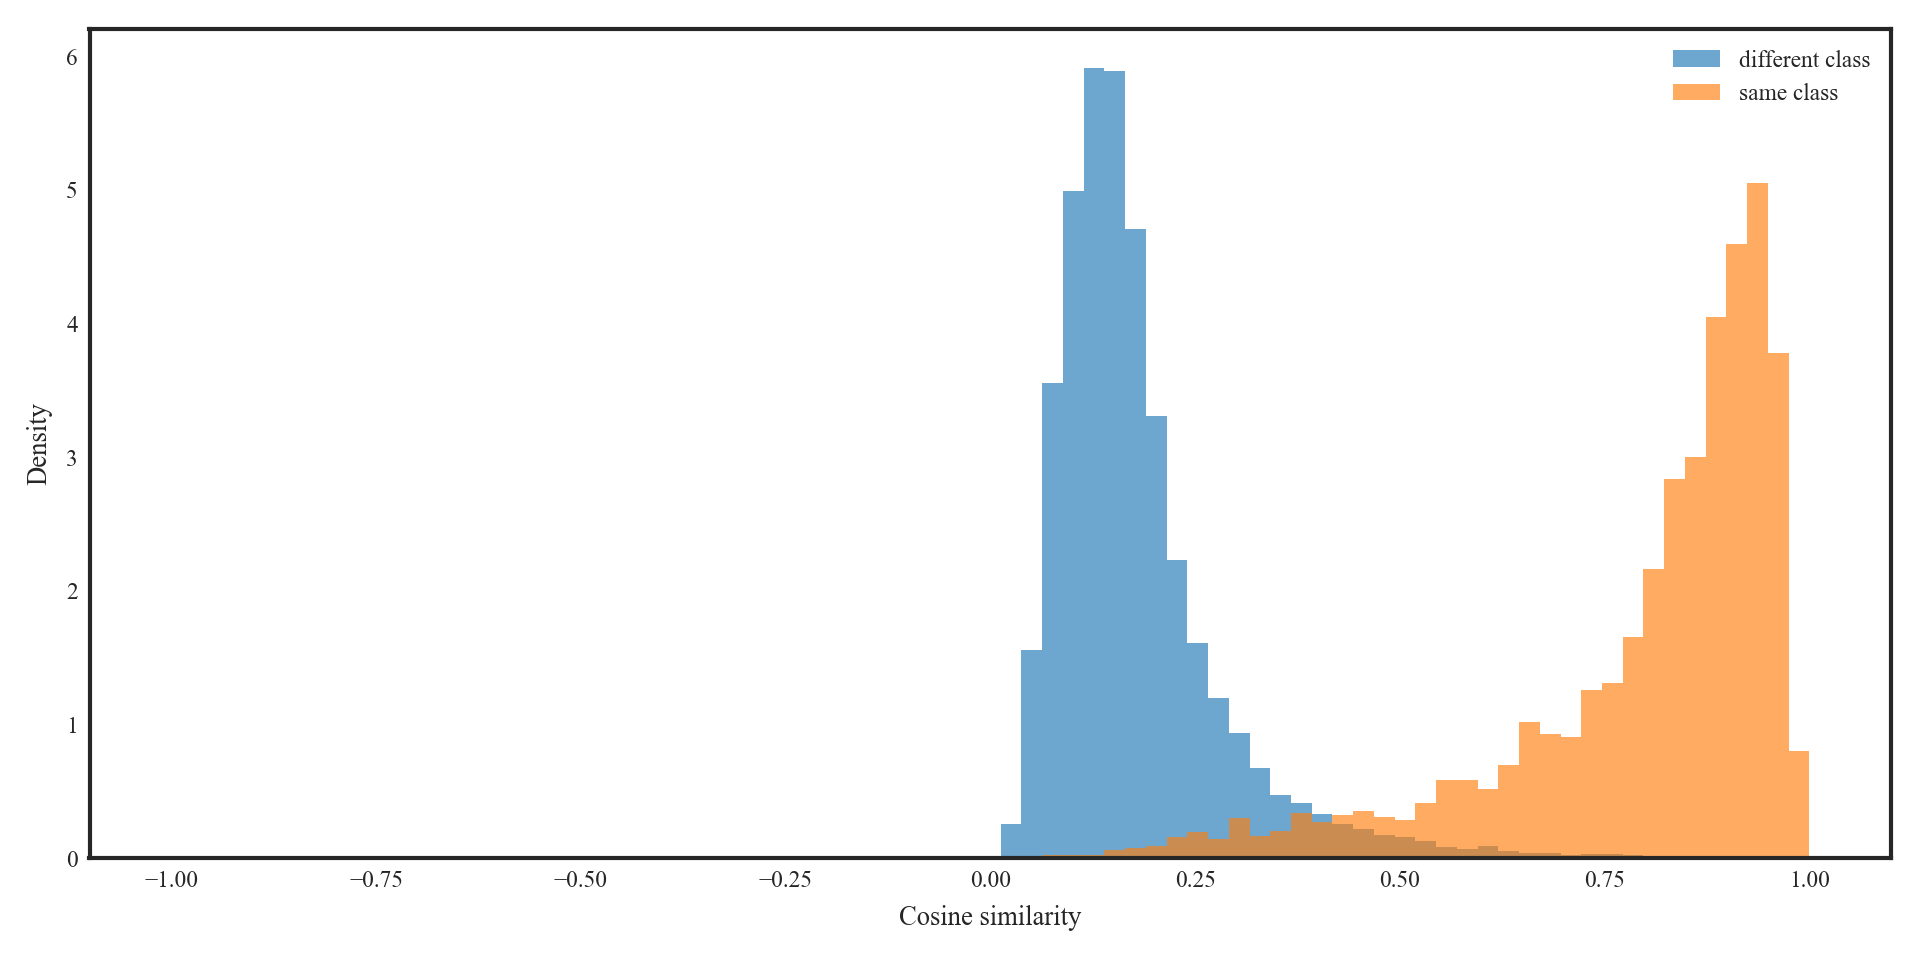
\includegraphics[width=0.55\linewidth]{v12_standard_setup_terel_baseline/pairwise_cosine_distribution.png}
  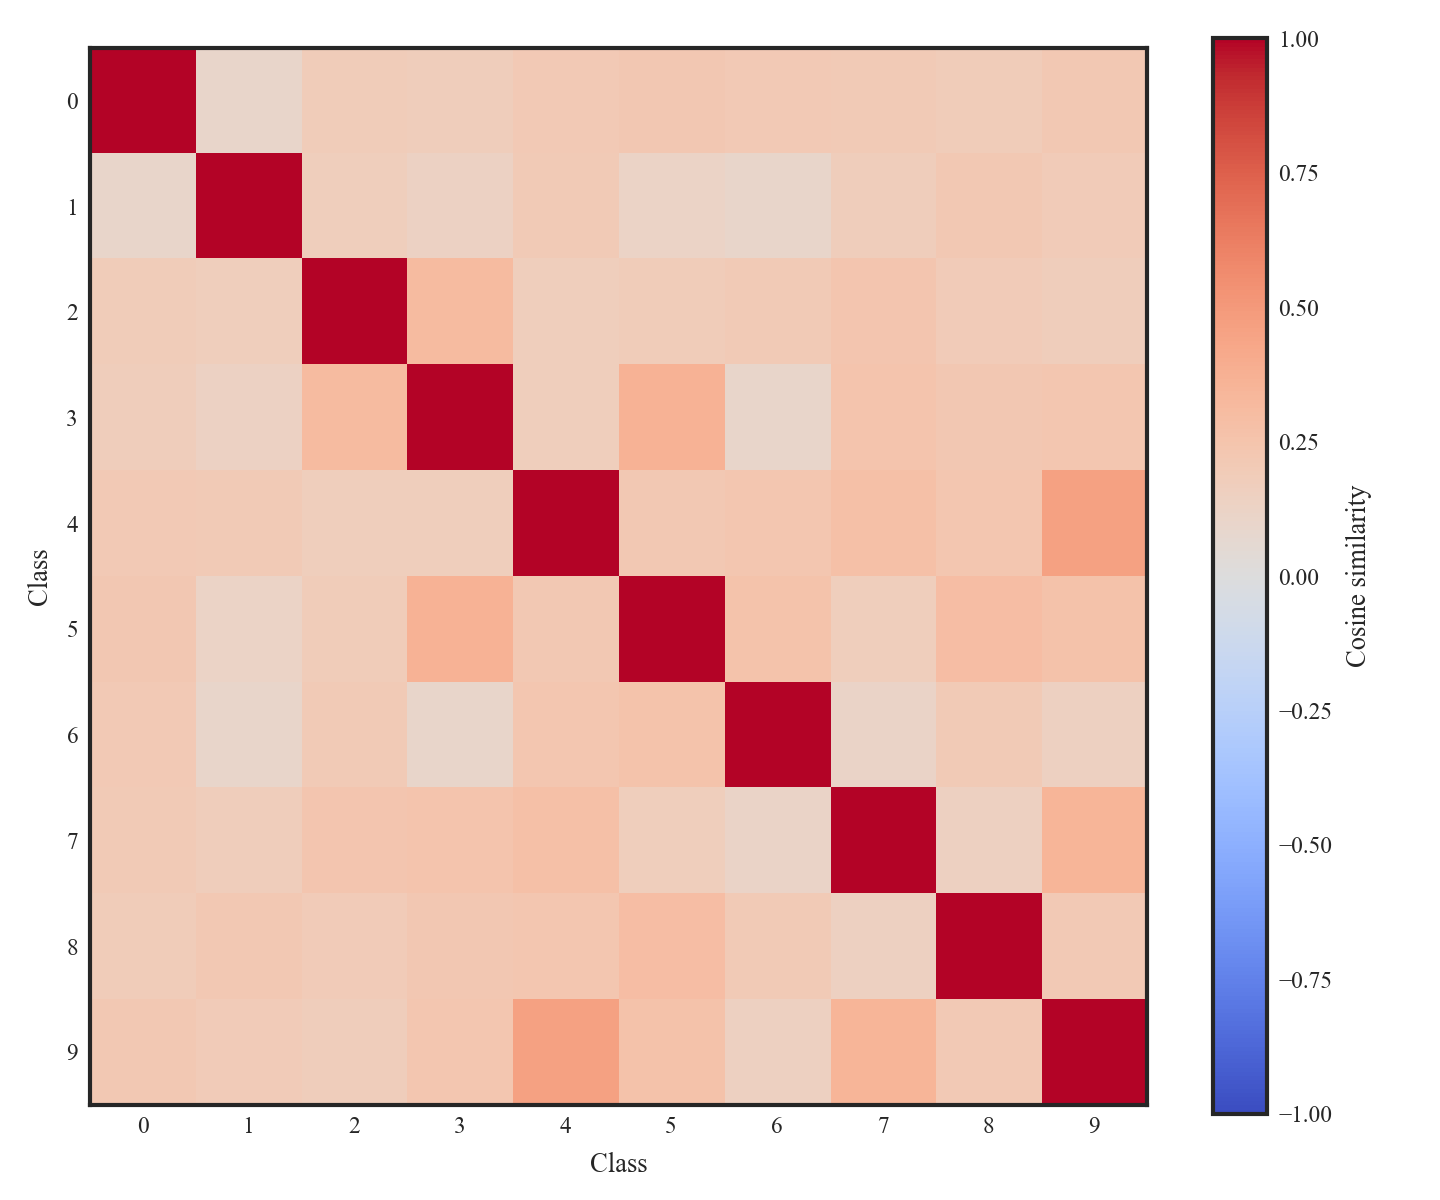
\includegraphics[width=0.32\linewidth]{v12_standard_setup_terel_baseline/class_prototype_cosine.png}
  \caption{Cosine similarity diagnostics for TeReL representations. \textbf{Left:} Pairwise cosine similarity distribution for same-class vs.\ different-class pairs. \textbf{Right:} Cosine similarity matrix of class prototype vectors (class-mean latent embeddings).}
  \label{fig:cosine_overlap_and_pairs}
\end{figure}
\FloatBarrier

\paragraph{Hypothesis 2: early features are rich and non-trivial.}
To assess whether TeReL learns meaningful low-level features, Figure~\ref{fig:first_layer_top64_rf} visualizes the top-64 first-layer receptive fields by weight $\ell_2$ norm. Some resemble oriented stroke detectors; many appear to encode more complex templates or mass-distribution patterns, suggesting that TeReL induces a diverse and structured first-layer feature basis.

\begin{figure}[!ht]
  \centering
  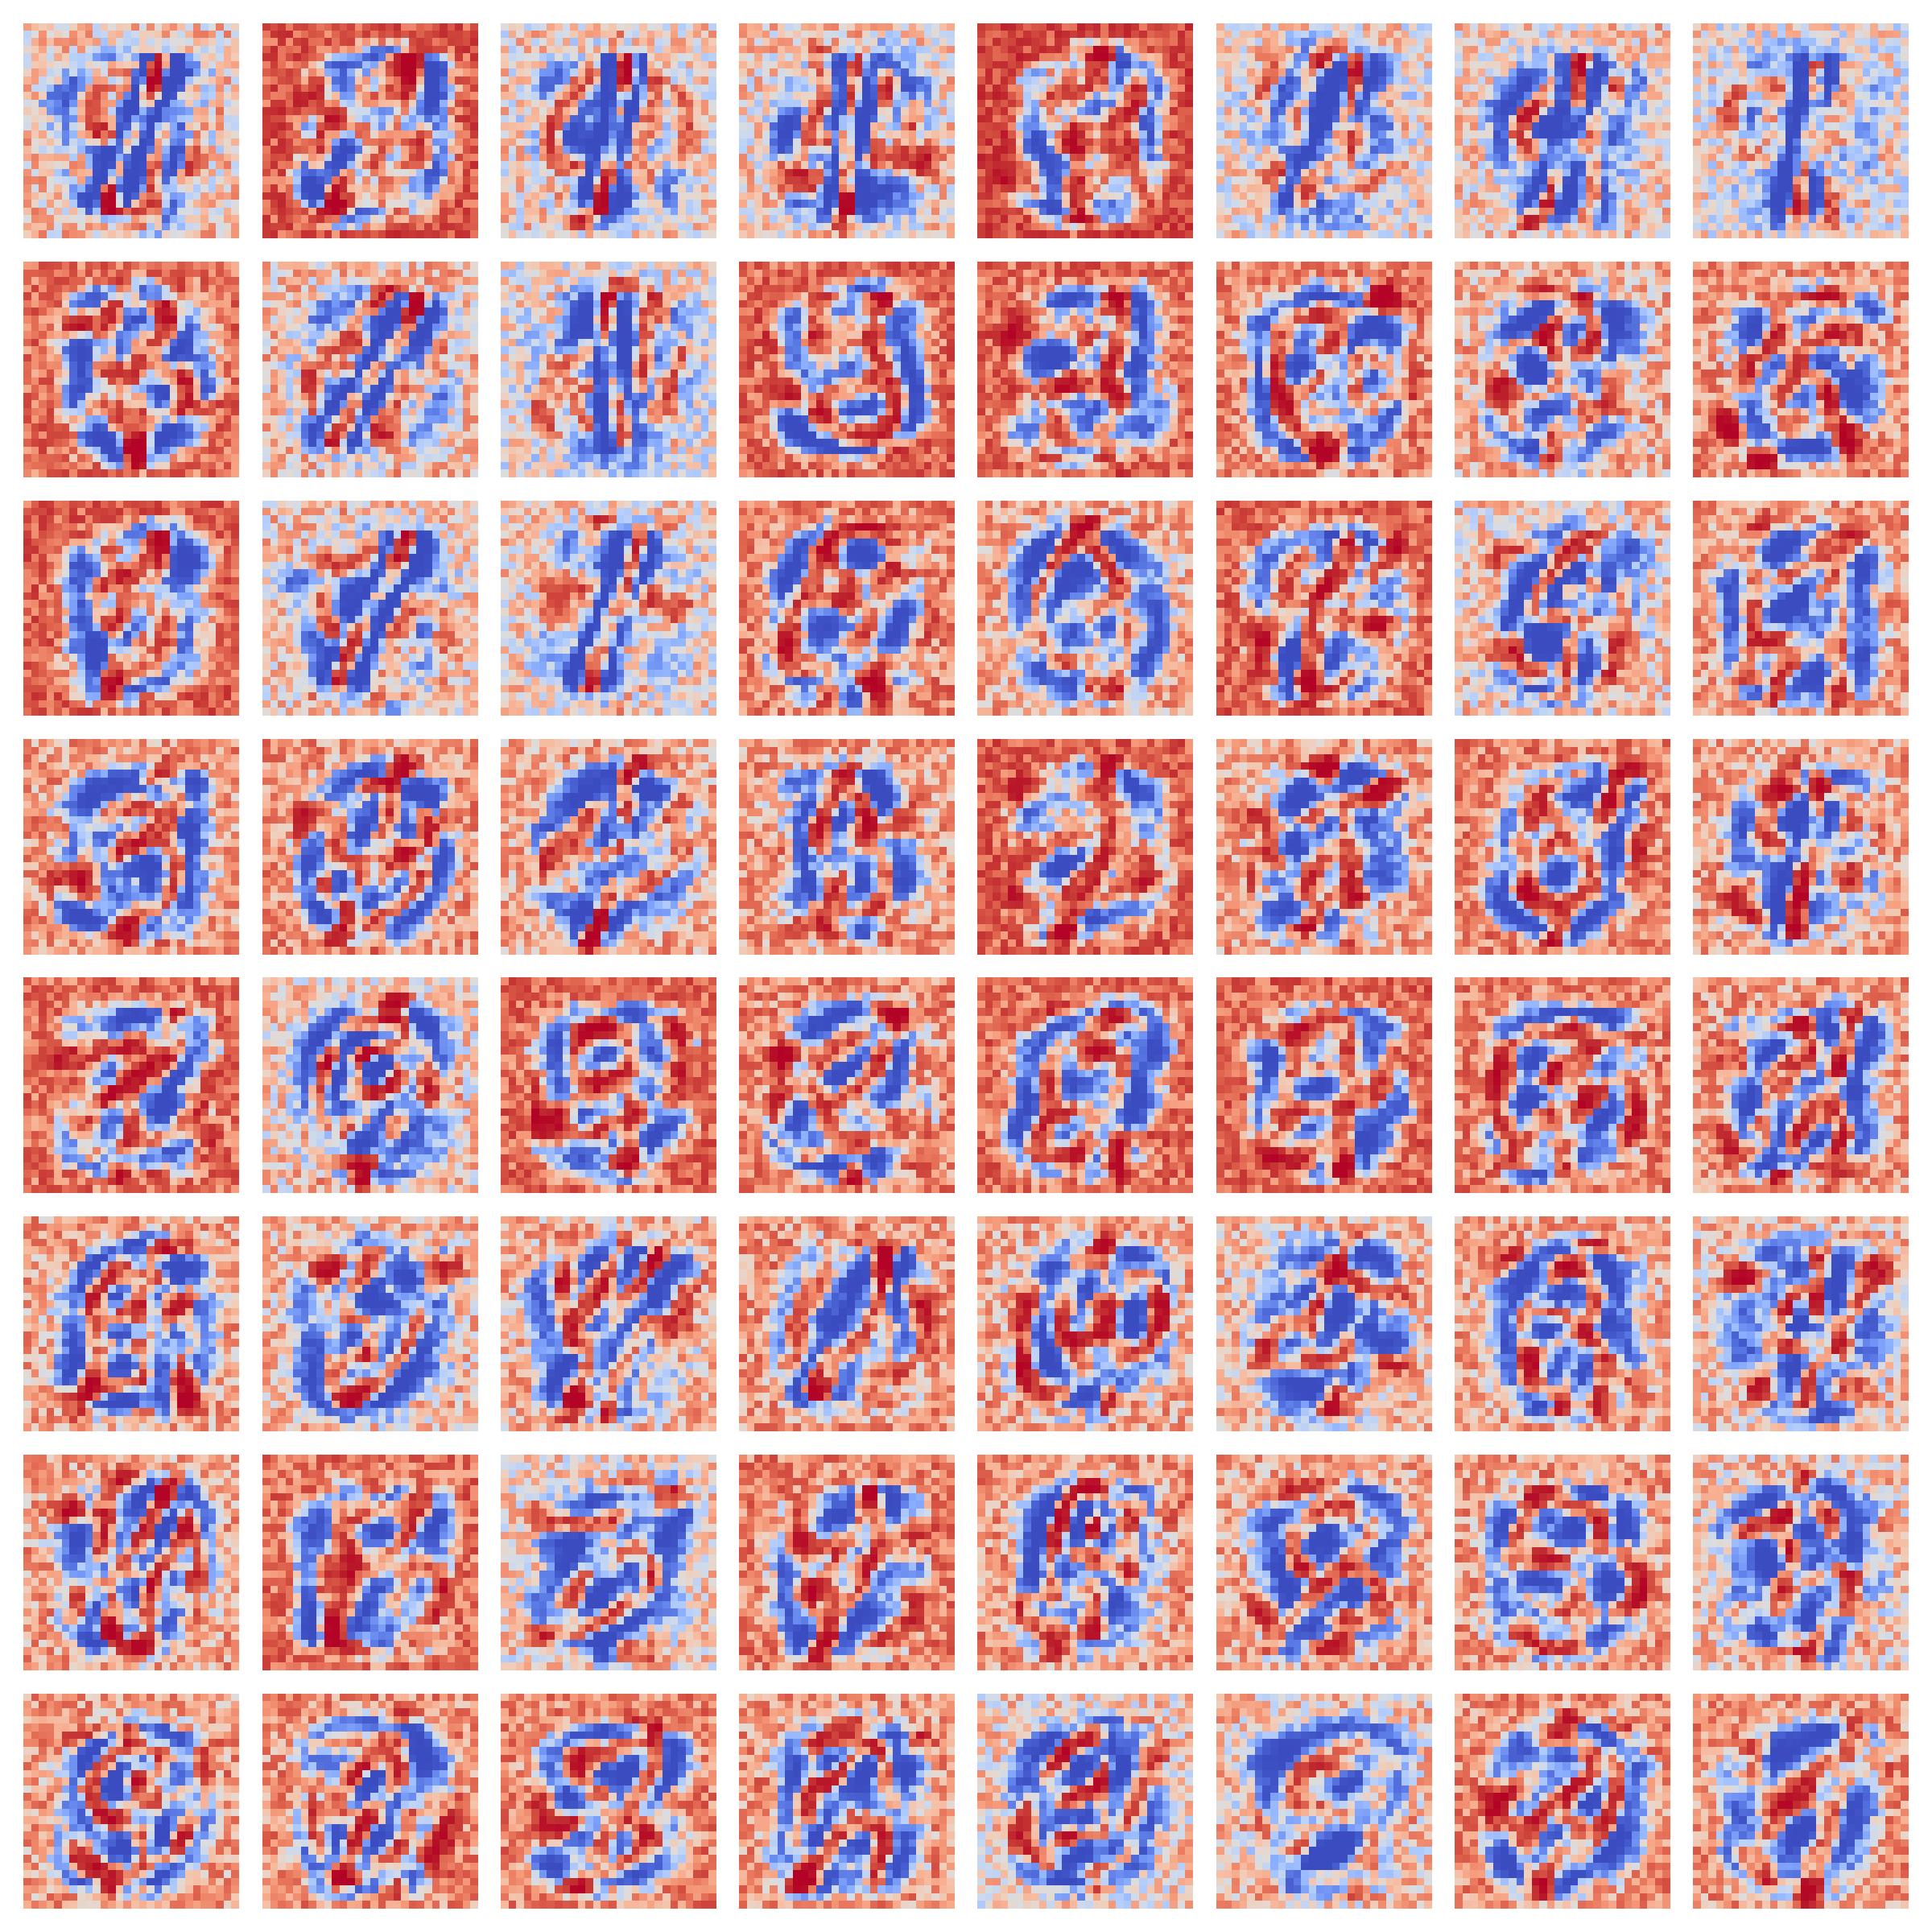
\includegraphics[width=0.78\linewidth]{v12_standard_setup_terel_baseline/first_layer_top64_rf.png}
  \caption{Top-64 first-layer receptive fields selected by weight $\ell_2$ norm.}
  \label{fig:first_layer_top64_rf}
\end{figure}
\FloatBarrier

\paragraph{Hypothesis 3: neurons specialize.}
Figure~\ref{fig:top_selective_neurons_heatmap} reports class-conditional mean activations for the most selective neurons. Several neurons clearly specialize, activating strongly for particular digits while remaining comparatively inactive for others, which is consistent with a representation that contains class-informative features.

\begin{figure}[!ht]
  \centering
  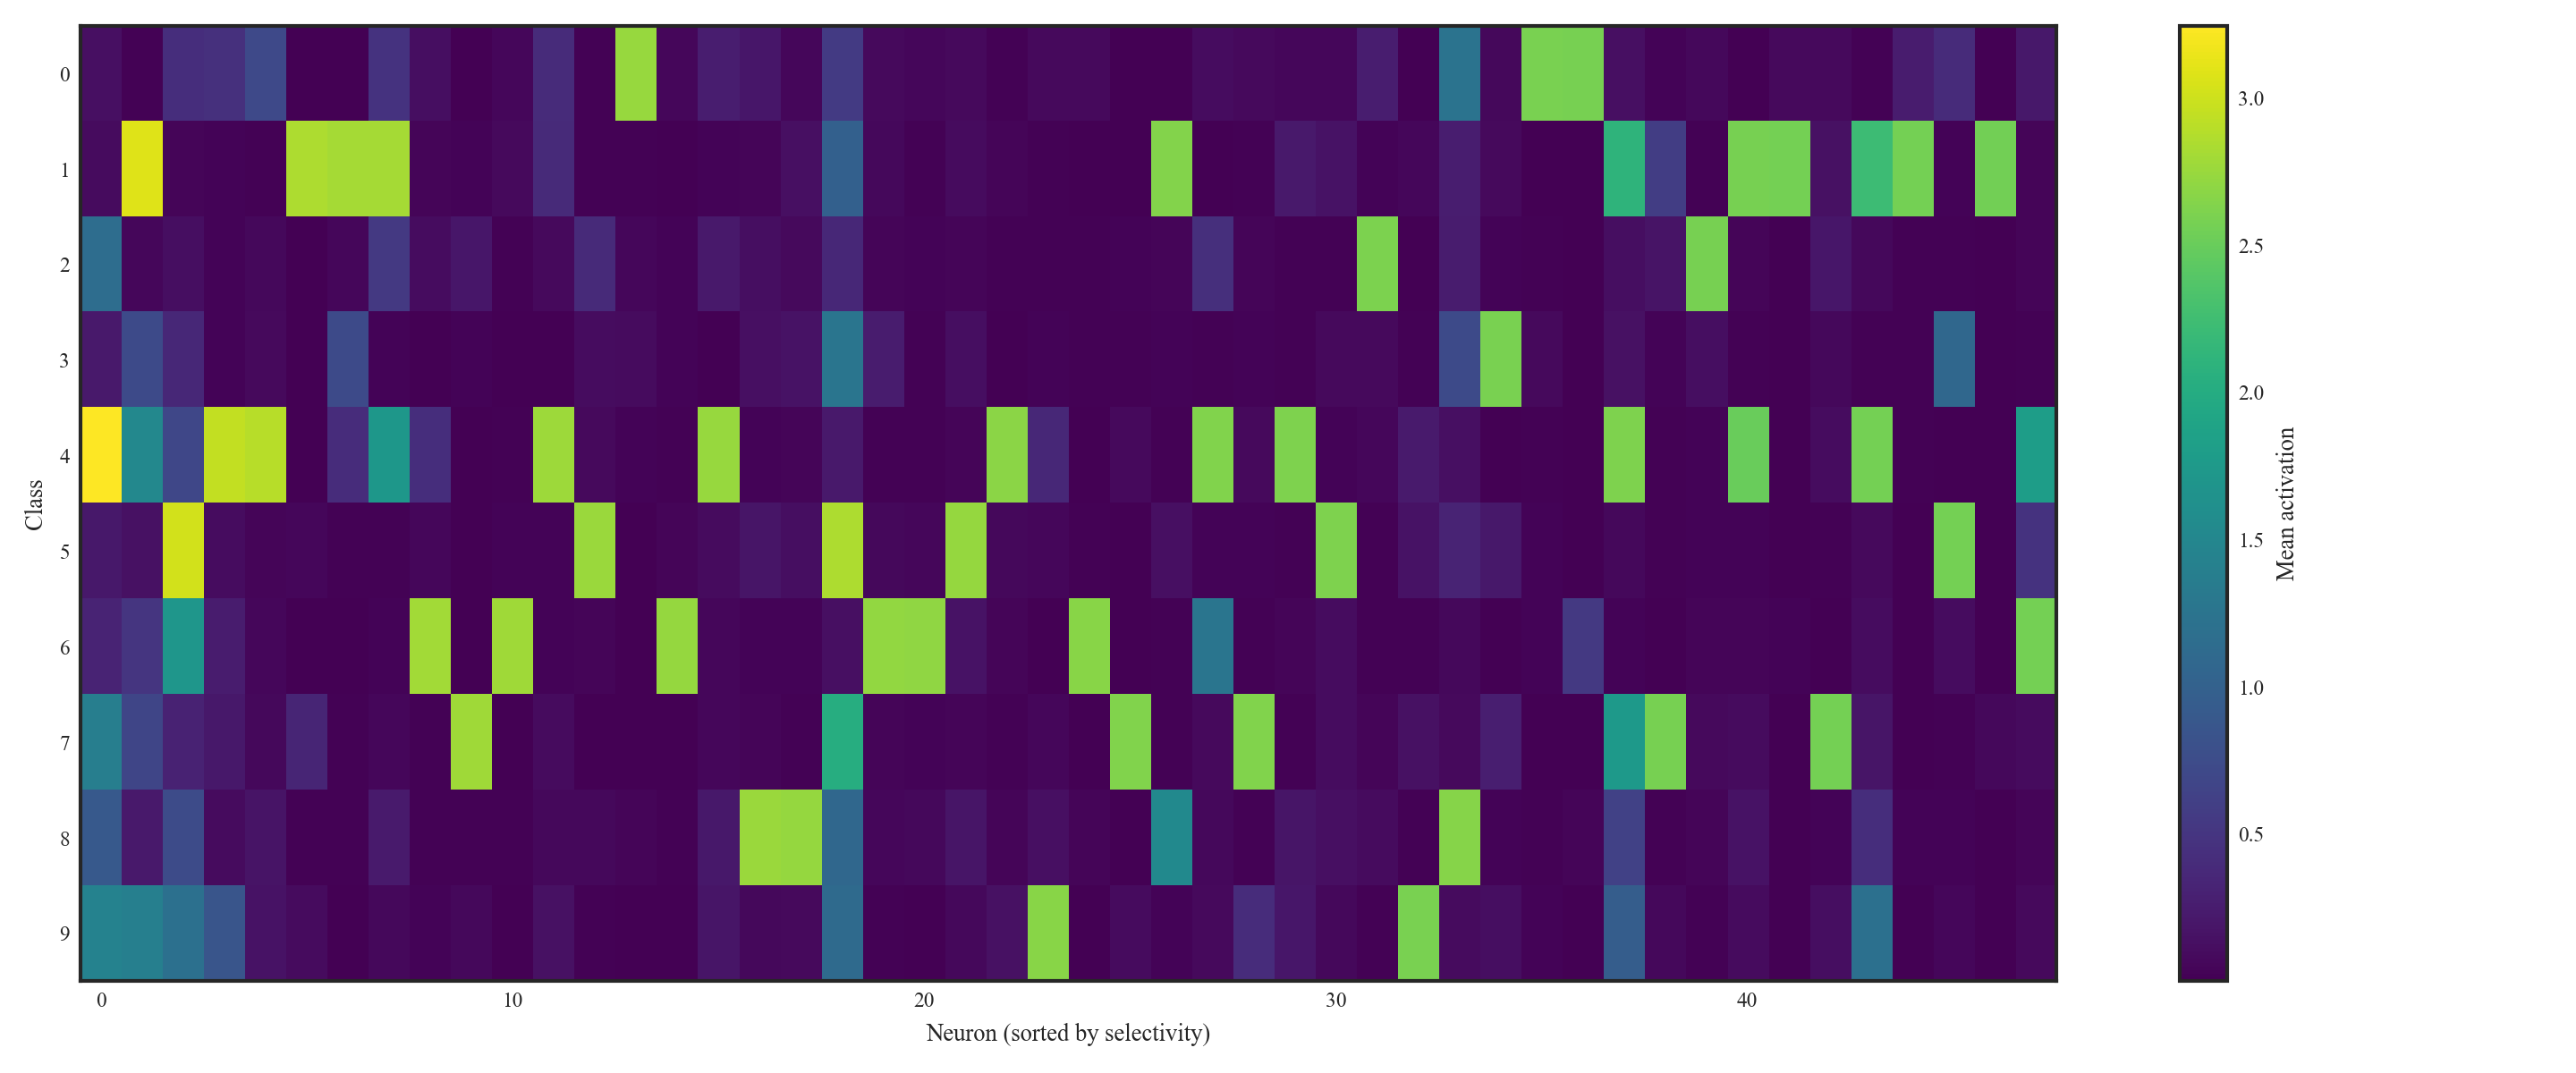
\includegraphics[width=0.675\linewidth]{v12_standard_setup_terel_baseline/top_selective_neurons_heatmap.png}
  \caption{Class-conditional mean activations for the most selective neurons.}
  \label{fig:top_selective_neurons_heatmap}
\end{figure}
\FloatBarrier

\paragraph{Hypothesis 4: local neighborhood structure is consistent.}
Figure~\ref{fig:spectral_representations} shows a Laplacian-eigenmap (spectral) projection built from a cosine $k$-nearest-neighbor graph over latent vectors. The embedding reveals class-consistent local neighborhoods, indicating that nearby representations correspond to the same digit.

\begin{figure}[!ht]
  \centering
  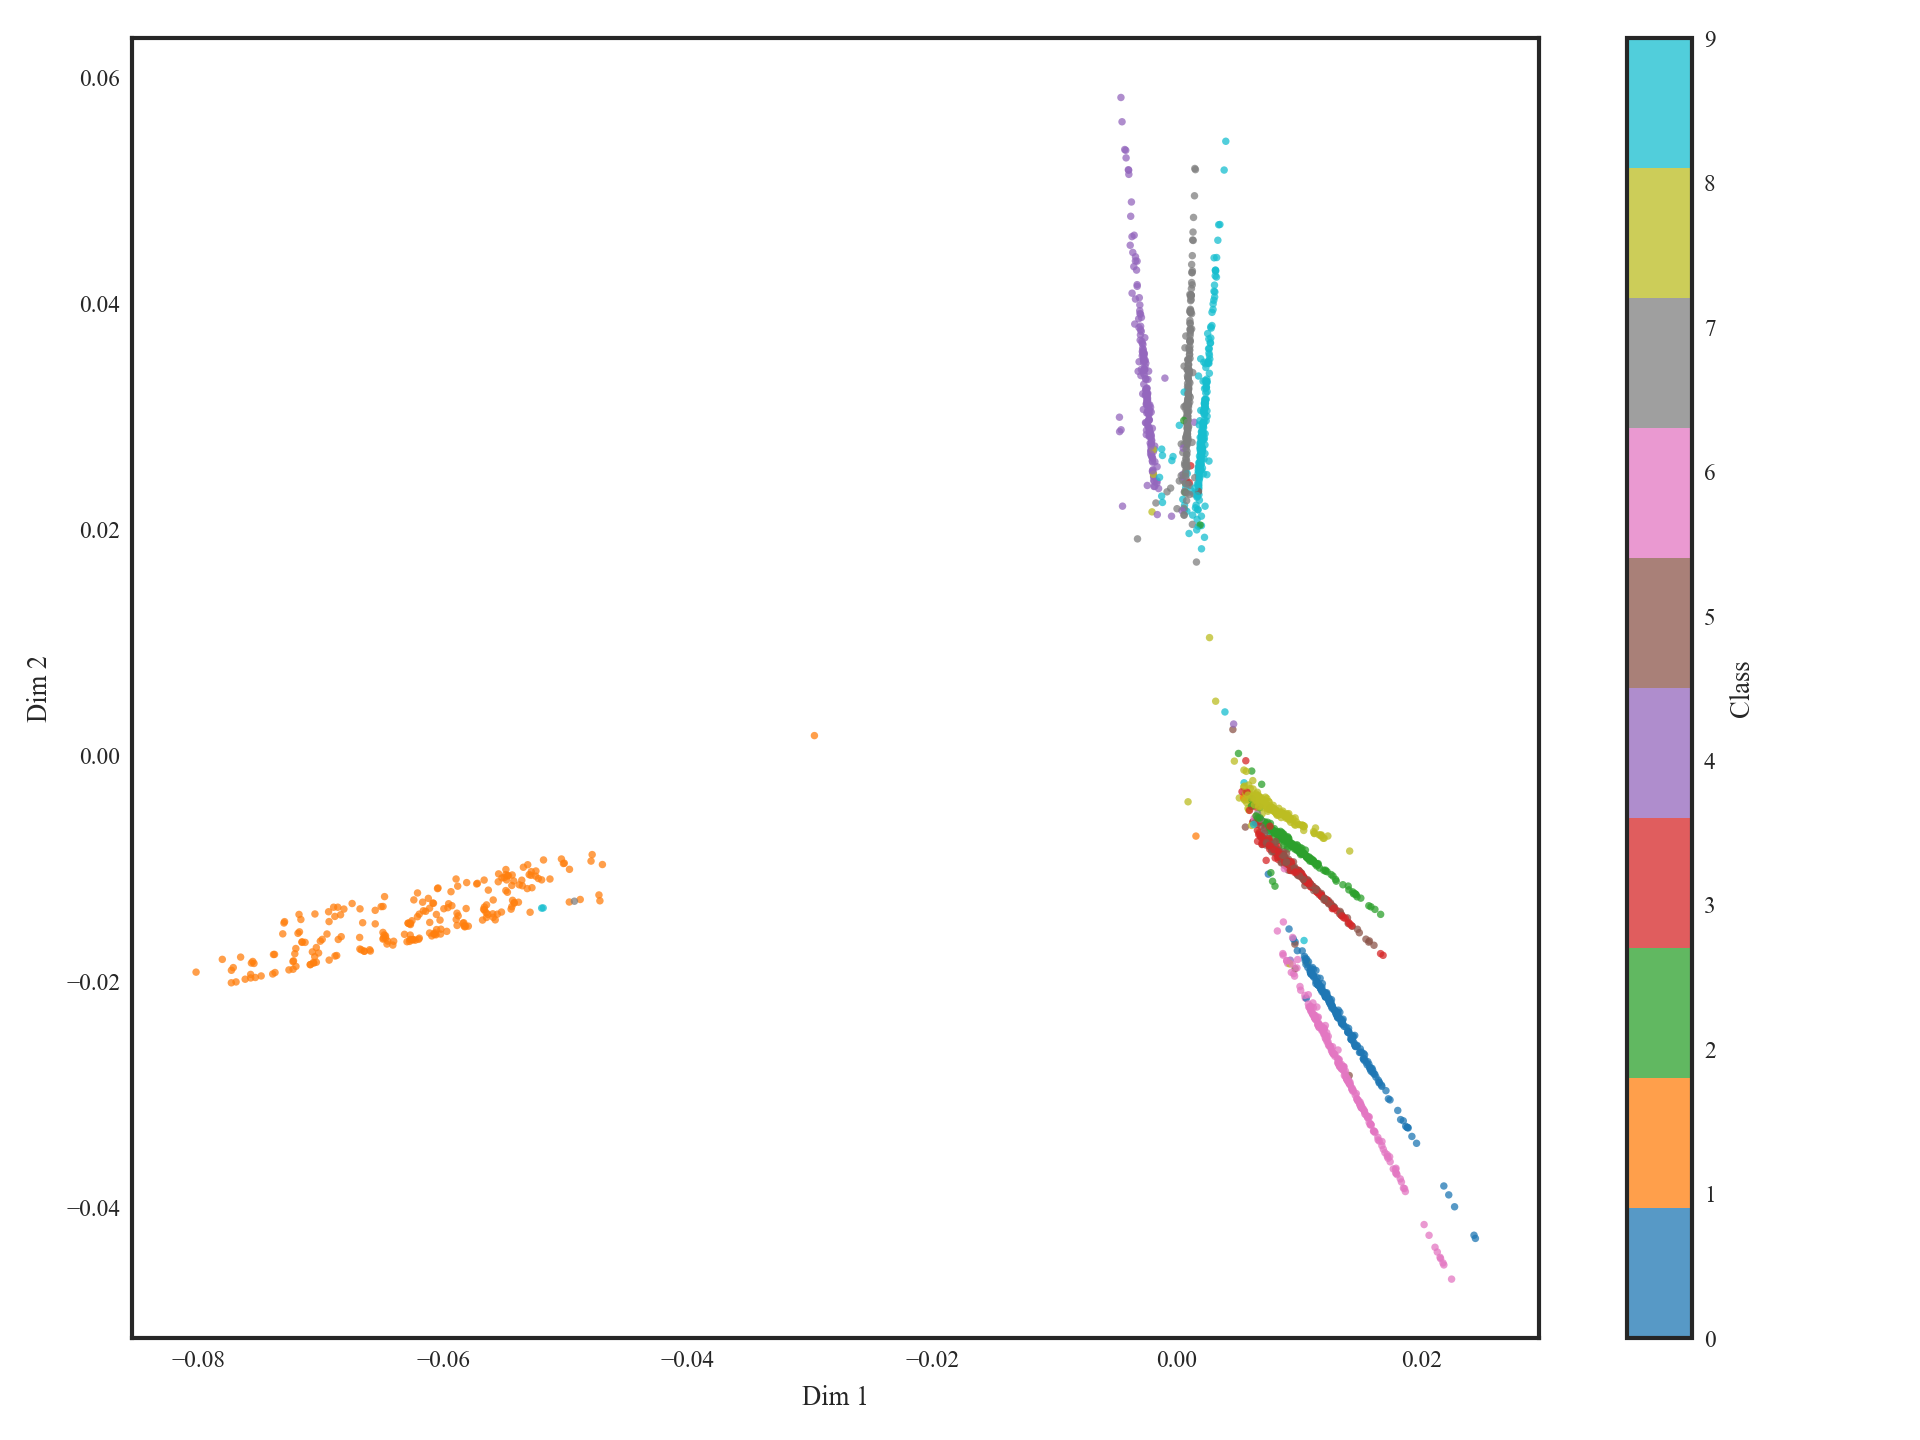
\includegraphics[width=0.52\linewidth]{v12_standard_setup_terel_baseline/spectral_representations.png}
  \caption{Laplacian-eigenmap (spectral) projection of latent vectors based on a cosine $k$-nearest-neighbor graph.}
  \label{fig:spectral_representations}
\end{figure}
\FloatBarrier


%\paragraph{Linear-head errors by class.}
%For completeness, Figure~\ref{fig:confusion_matrix_normalized} shows the row-normalized confusion matrix of the linear head on validation data. Errors are not visible after normalizing the rows.

%\begin{figure}[!ht]
%  \centering
%  % Smaller confusion matrix (as requested)
%  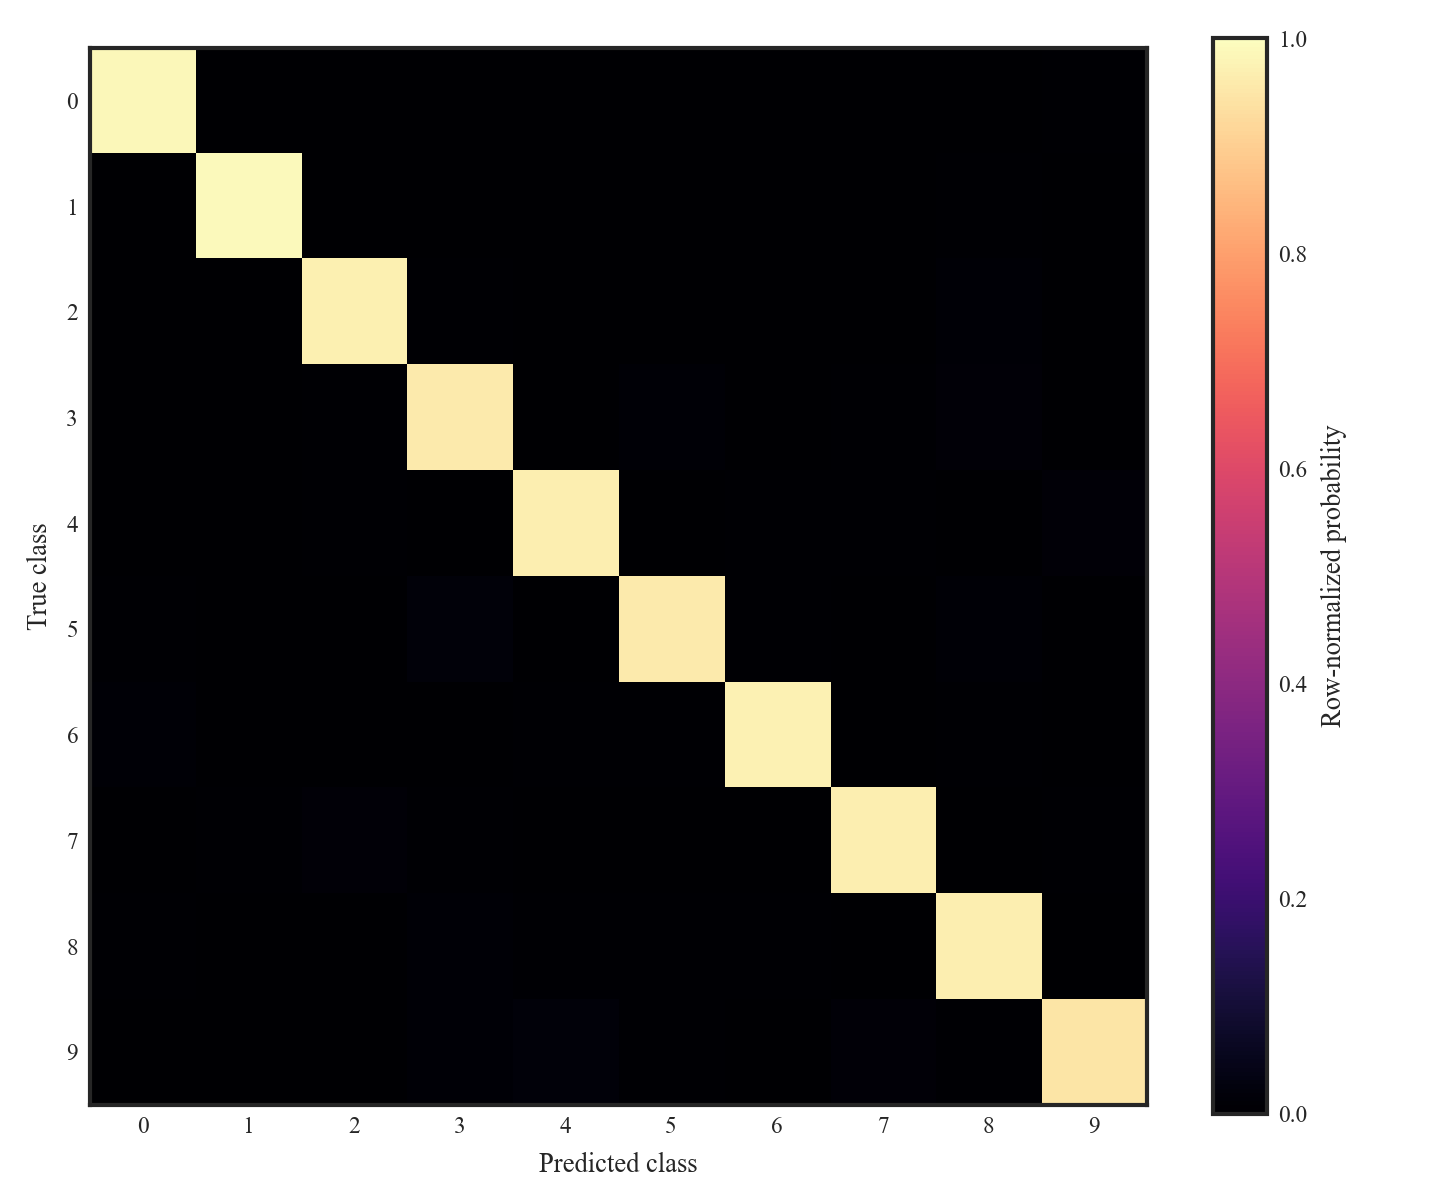
\includegraphics[width=0.38\linewidth]{v12_standard_setup_terel_baseline/confusion_matrix_normalized.png}
%  \caption{Row-normalized confusion matrix of linear-head predictions on validation data.}
%  \label{fig:confusion_matrix_normalized}
%\end{figure}

\subsection{Findings and ablations}\label{sec:ablations}
\noindent Detailed ablation tables and run specifications are provided in Appendix~\ref{app:ablation-results}. We go over the most important findings here.

An untrained encoder with the 512 by 256 layout yields approximately 90\% validation accuracy when a linear head is trained, in batches, on last layer's activations. We use this figure as a baseline threshold; any encoder whose linear head accuracy falls substantially below this threshold is considered to be in failure mode.

Ablation of any single TeReL loss term reduces peak performance to at most seventy percent in batched offline experiments, showing that all terms are necessary, even for small-scale networks.
Activation function changes from ReLU to tanh or sigmoid reduce accuracy by less than four percentage points in the tested configurations. Using the GeLU activation function improved performance \cite{hendrycks2016}.

The covariance objective depends on second moments, so training the lateral module and reducing the off-diagonal energy can interact strongly with the effective handling of second-moment statistics by the optimizer. In our experiments, adaptive optimizers that track second moments (e.g., Adam) produced stable covariance minimization in TeReL runs. \cite{kingma2014, wilson2017}
In contrast, standard stochastic gradient descent with momentum often failed to minimize the lateral covariance term reliably in our setup. A representative SGD run that used the lateral module reached 93\% test accuracy for one seed, but further tuning did not close the gap to Adam-based TeReL runs. This optimizer interaction should be considered an implementation constraint when choosing whether to use a learned lateral layer or to rely on direct covariance estimates.

We observe that the learned lateral layer creates an optimization landscape that benefits from optimizers capable of handling second moment structure. In our runs, Adam achieves stable covariance minimization with covariance loss magnitudes around one to two at steady state. SGD with the lateral head tended to produce much larger covariance loss values, in the order of dozens, and poorer final accuracy in the tested configurations: SGD runs achieve 92\% accuracy for TeReL at seed 42 when halving the variance coefficient. The empirical observations motivate us to recommend Adam for TeReL with lateral layers in the current implementation. 

Choosing the minimum variance $\tau$ as 1 yielded the best performance. Using a random distribution of $\tau$ for different neurons did not improve performance either.
Chunk size is critical: A run with the TeReL setup without batchnorm with a chunk size of 8 yielded validation accuracy of 96.68\% after 20 epochs, which is significantly lower than for a chunk size of 16. A run with chunk\_size=32 achieves achieves 93.98\% accuracy.

% RNN / sequence prediction section (MNIST-Rows)
% Intended insertion point: after the MNIST experiments section.

\section{Sequence prediction on MNIST-Rows}\label{sec:mnist_rows_rnn}

We evaluate whether TeReL can be extended to a simple recurrent setting under a locality constraint. The task is \texttt{mnist-rows}: given an image row sequence, the model predicts the next row in a one-step autoregressive objective ($x_t \rightarrow x_{t+1}$). We report validation one-step prediction mean squared error (MSE).

As a baseline, we compare against a backpropagation-trained recurrent model optimized with backpropagation through time (BPTT).

\subsection{Quantitative results}
We additionally report the per-timestep latent update magnitude $\lVert \Delta h \rVert_2 = \lVert h_t - h_{t-1} \rVert_2$ as a coarse summary of state dynamics. In this setup, TeReL yields larger step-to-step state changes than the backpropagation baseline (Table~\ref{tab:mnist_rows_one_step}), consistent with a more dynamic hidden-state trajectory over the sequence.

\begin{table}[h!]
  \centering
  \caption{One-step next-row prediction on \texttt{mnist-rows} (20 epochs). Lower MSE is better.}
  \begin{tabular}{lccc}
    \toprule
    \textbf{Model} & \textbf{Val.\ one-step MSE} & $\mathbf{\mu(\lVert \Delta h \rVert_2)}$ & $\mathbf{\sigma(\lVert \Delta h \rVert_2)}$ \\
    \midrule
    TeReL local-state + concat\_mlp & 0.22345 & 5.62 & 4.28 \\
    BP RNN baseline (MLP)        & 0.17569 & 4.06 & 2.80 \\
    \bottomrule
  \end{tabular}
  \label{tab:mnist_rows_one_step}
\end{table}

The TeReL sequence variant achieves substantially lower loss than earlier TeReL-RNN baselines in this project and serves as our primary TeReL sequence result; however, the backpropagation baseline remains better on pure one-step prediction loss.

In this section, we focus on one-step prediction as the primary evaluation target rather than long-horizon generation. We include multi-step autoregressive rollouts in the appendix to illustrate qualitative sequence prediction behavior.

Additional experimental details and qualitative rollouts are provided in Appendix~\ref{app:rnn-details}.

Additional experimental details and qualitative rollouts are provided in Appendix~\ref{app:rnn-details}.

\subsection{Latent trajectory visualization}
To compare the learned sequence dynamics, we visualize per-timestep latents with t-SNE and summarize mean latent trajectories across timesteps. Each TeReL plot is placed side-by-side with the corresponding backpropagation baseline plot for direct visual comparison.

\begin{figure}[!ht]
  \centering
  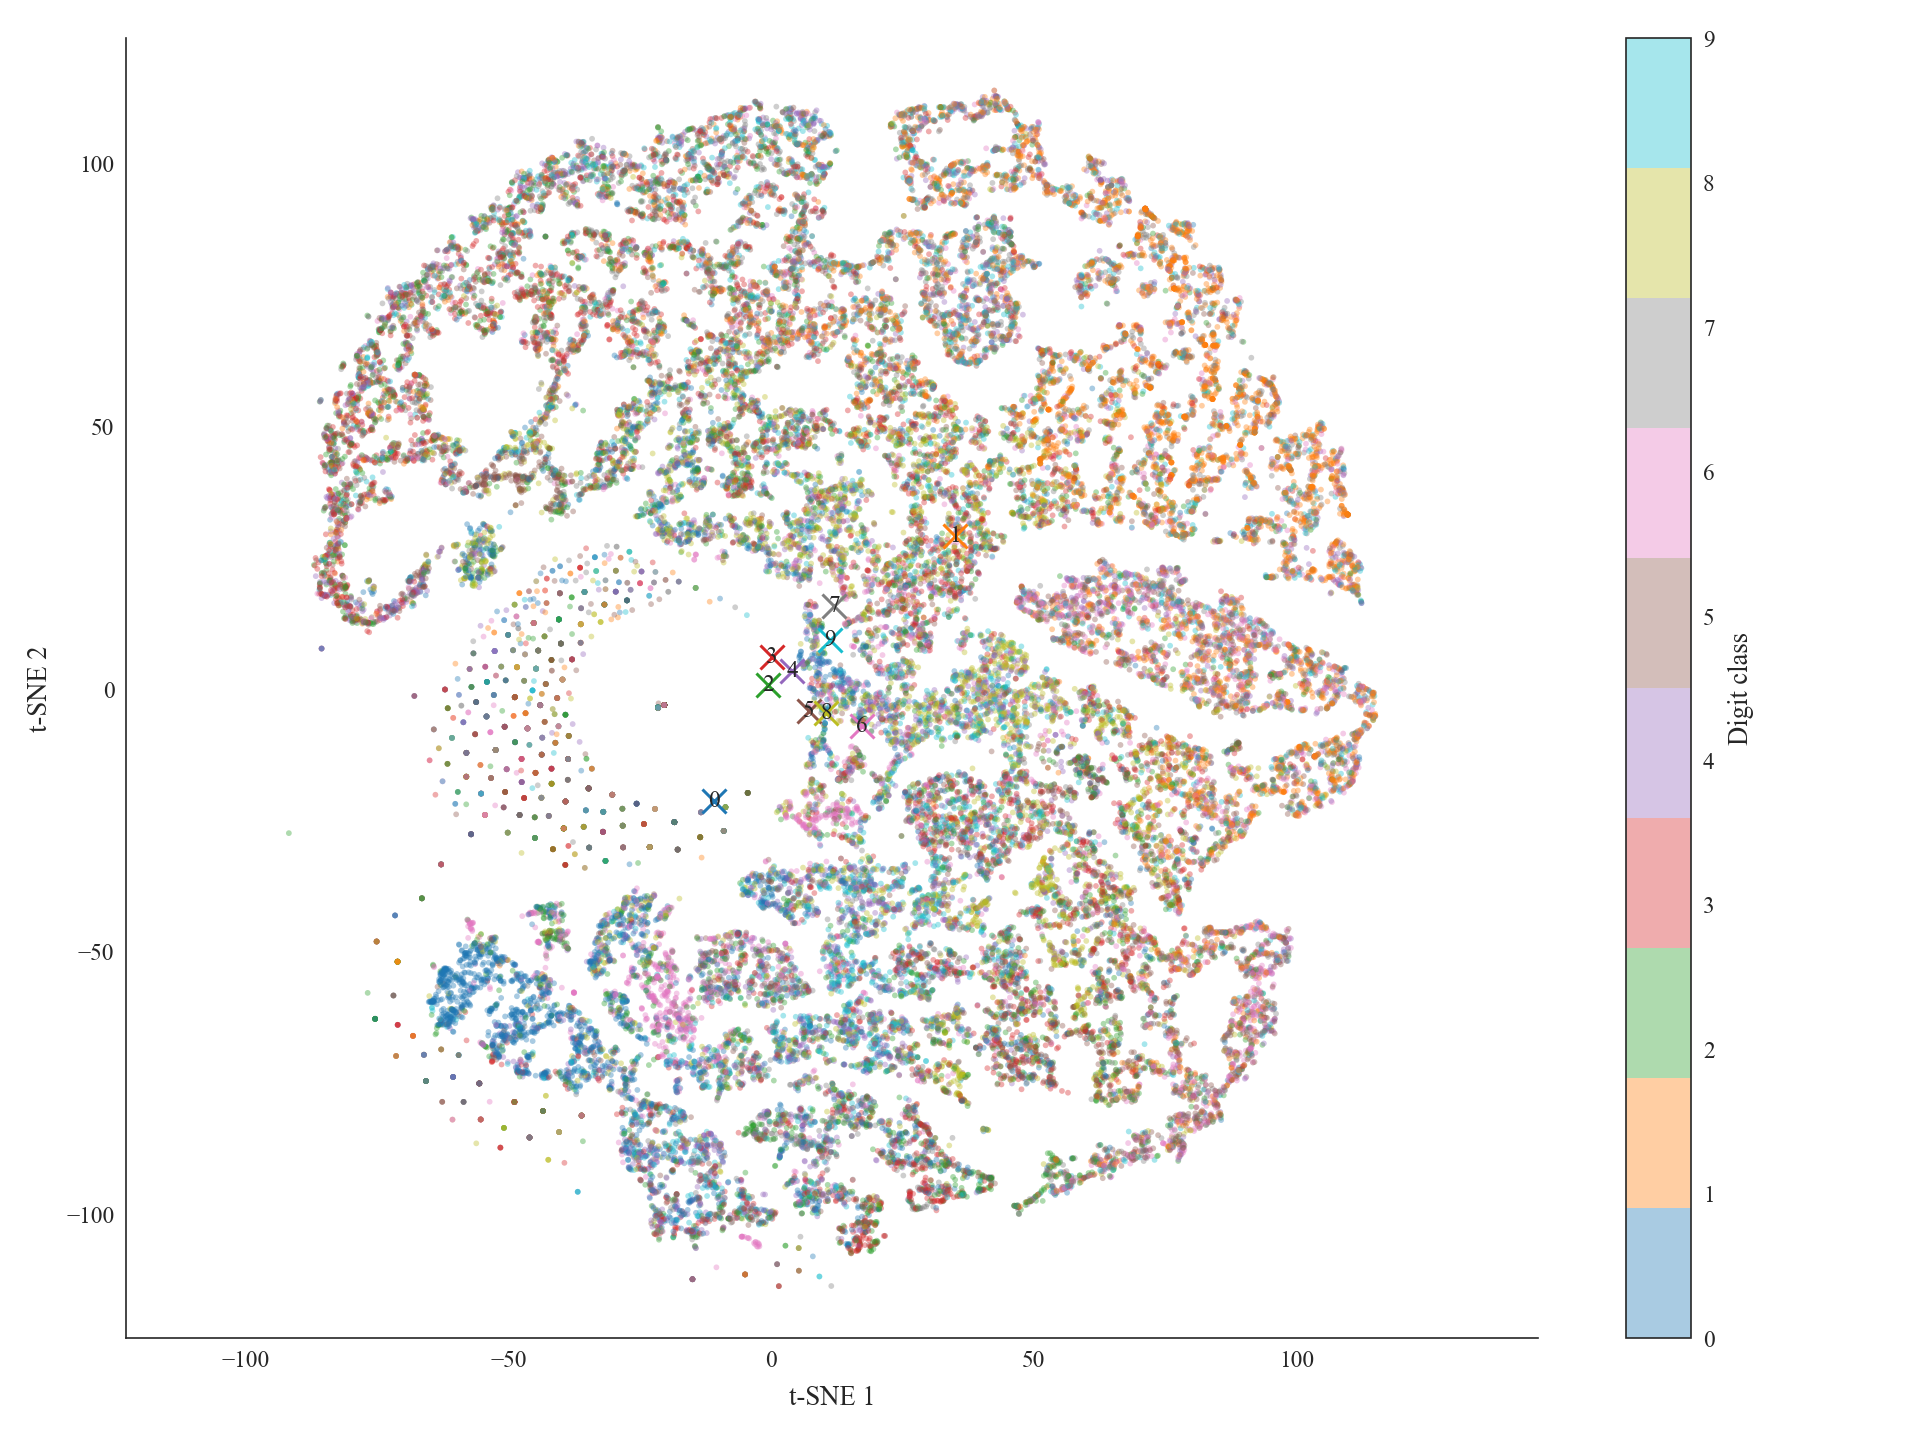
\includegraphics[width=0.49\linewidth]{terel_rnn_20ep/sequence_latent_tsne_samples.png}
  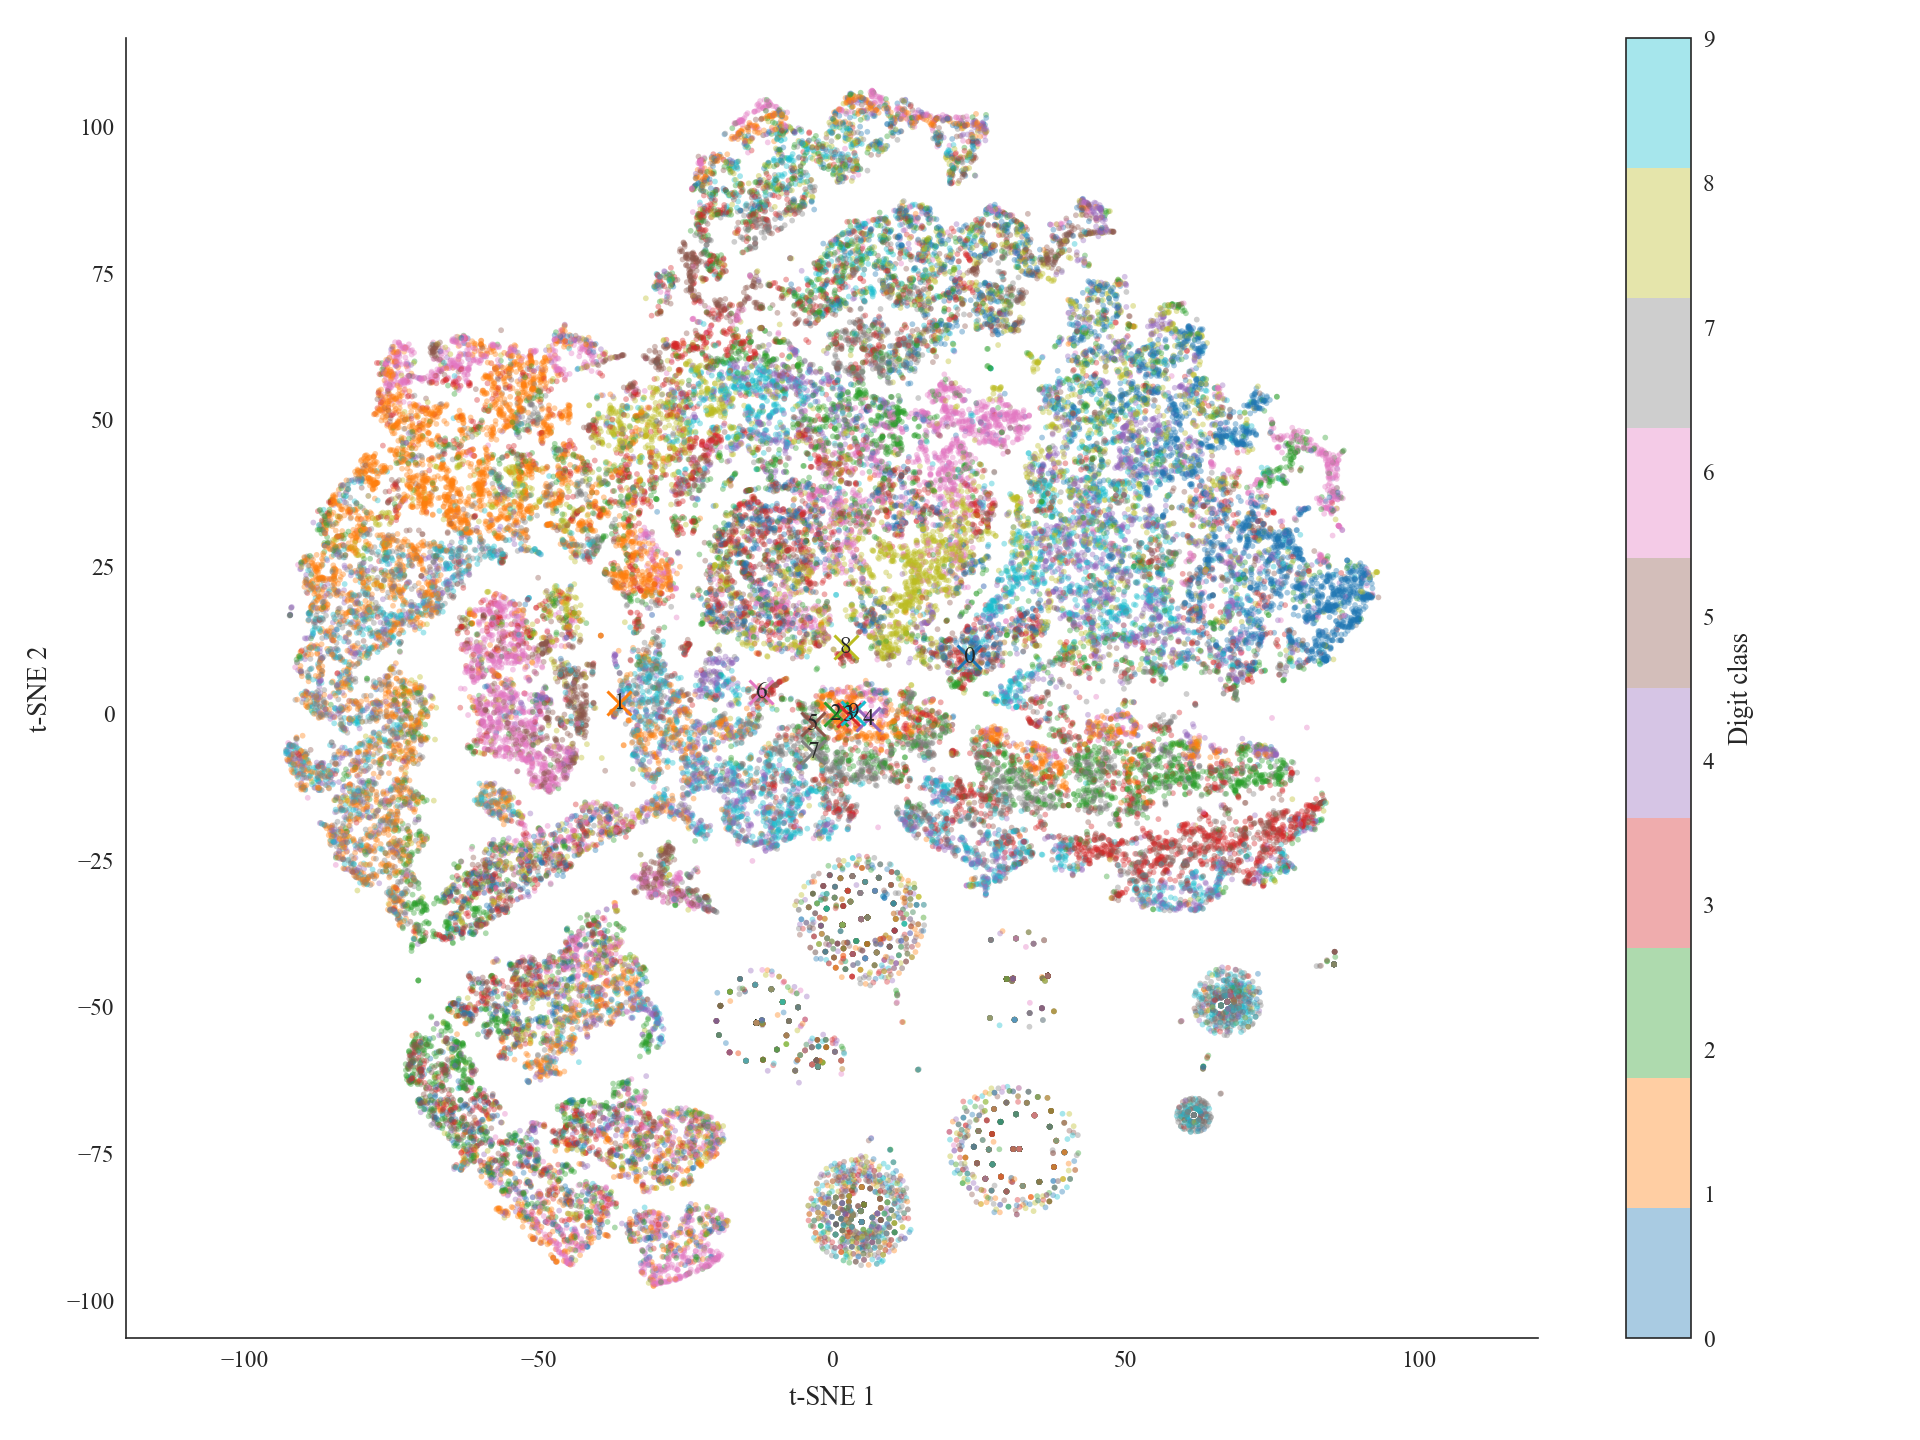
\includegraphics[width=0.49\linewidth]{bp_rnn_mnist_rows/sequence_latent_tsne_samples.png}
  \caption{t-SNE projection of per-timestep sequence latents. \textbf{Left:} TeReL. \textbf{Right:} BP.}
  \label{fig:mnist_rows_tsne_samples}
\end{figure}
\FloatBarrier

\begin{figure}[!ht]
  \centering
  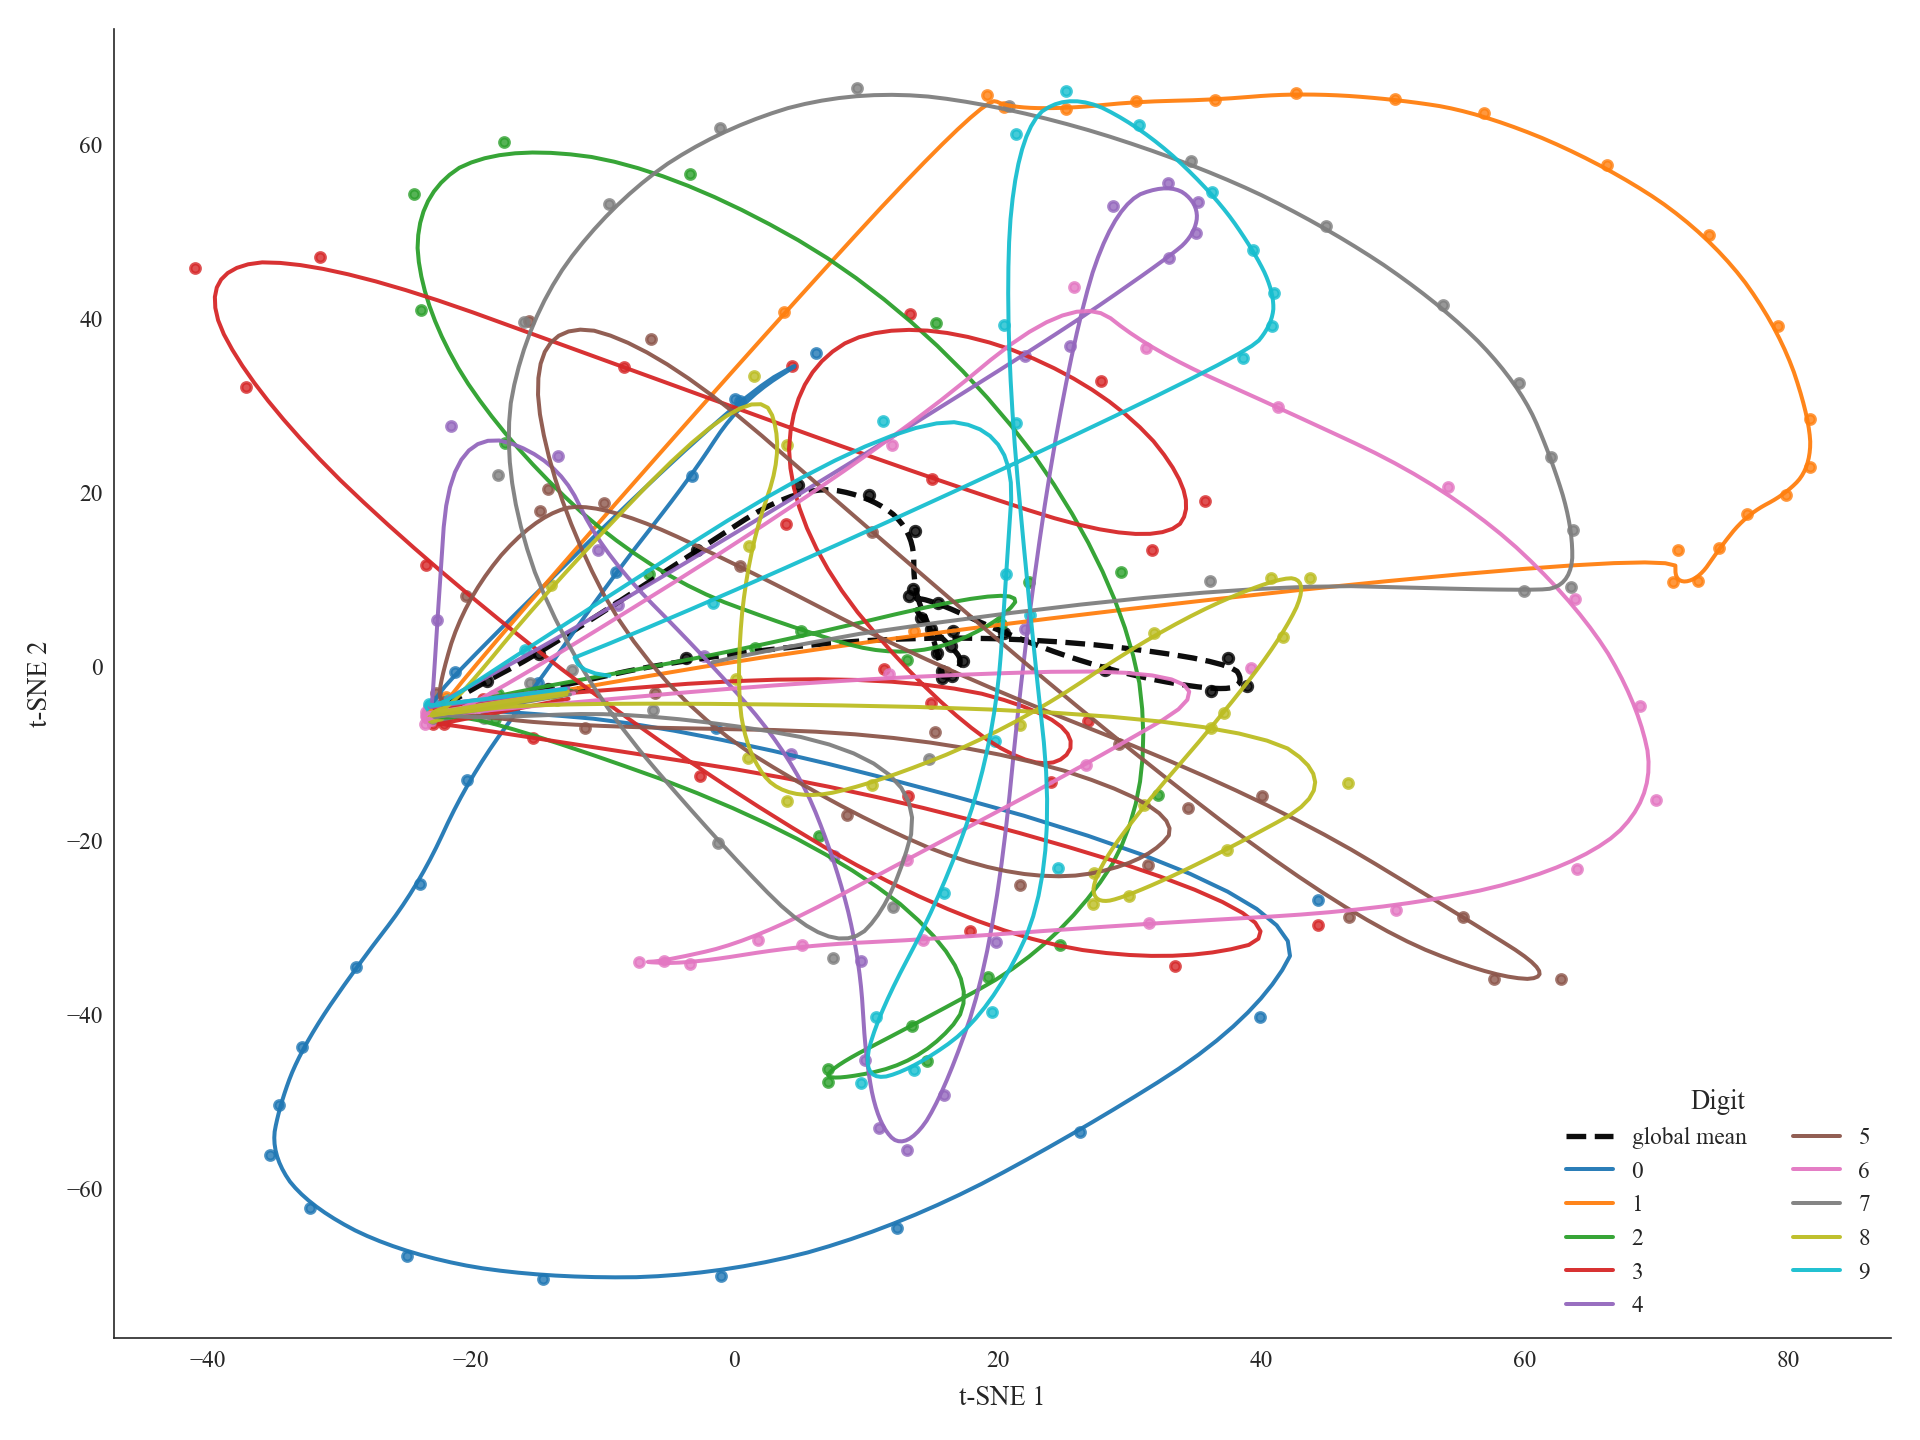
\includegraphics[width=0.49\linewidth]{terel_rnn_20ep/sequence_latent_tsne_mean_paths.png}
  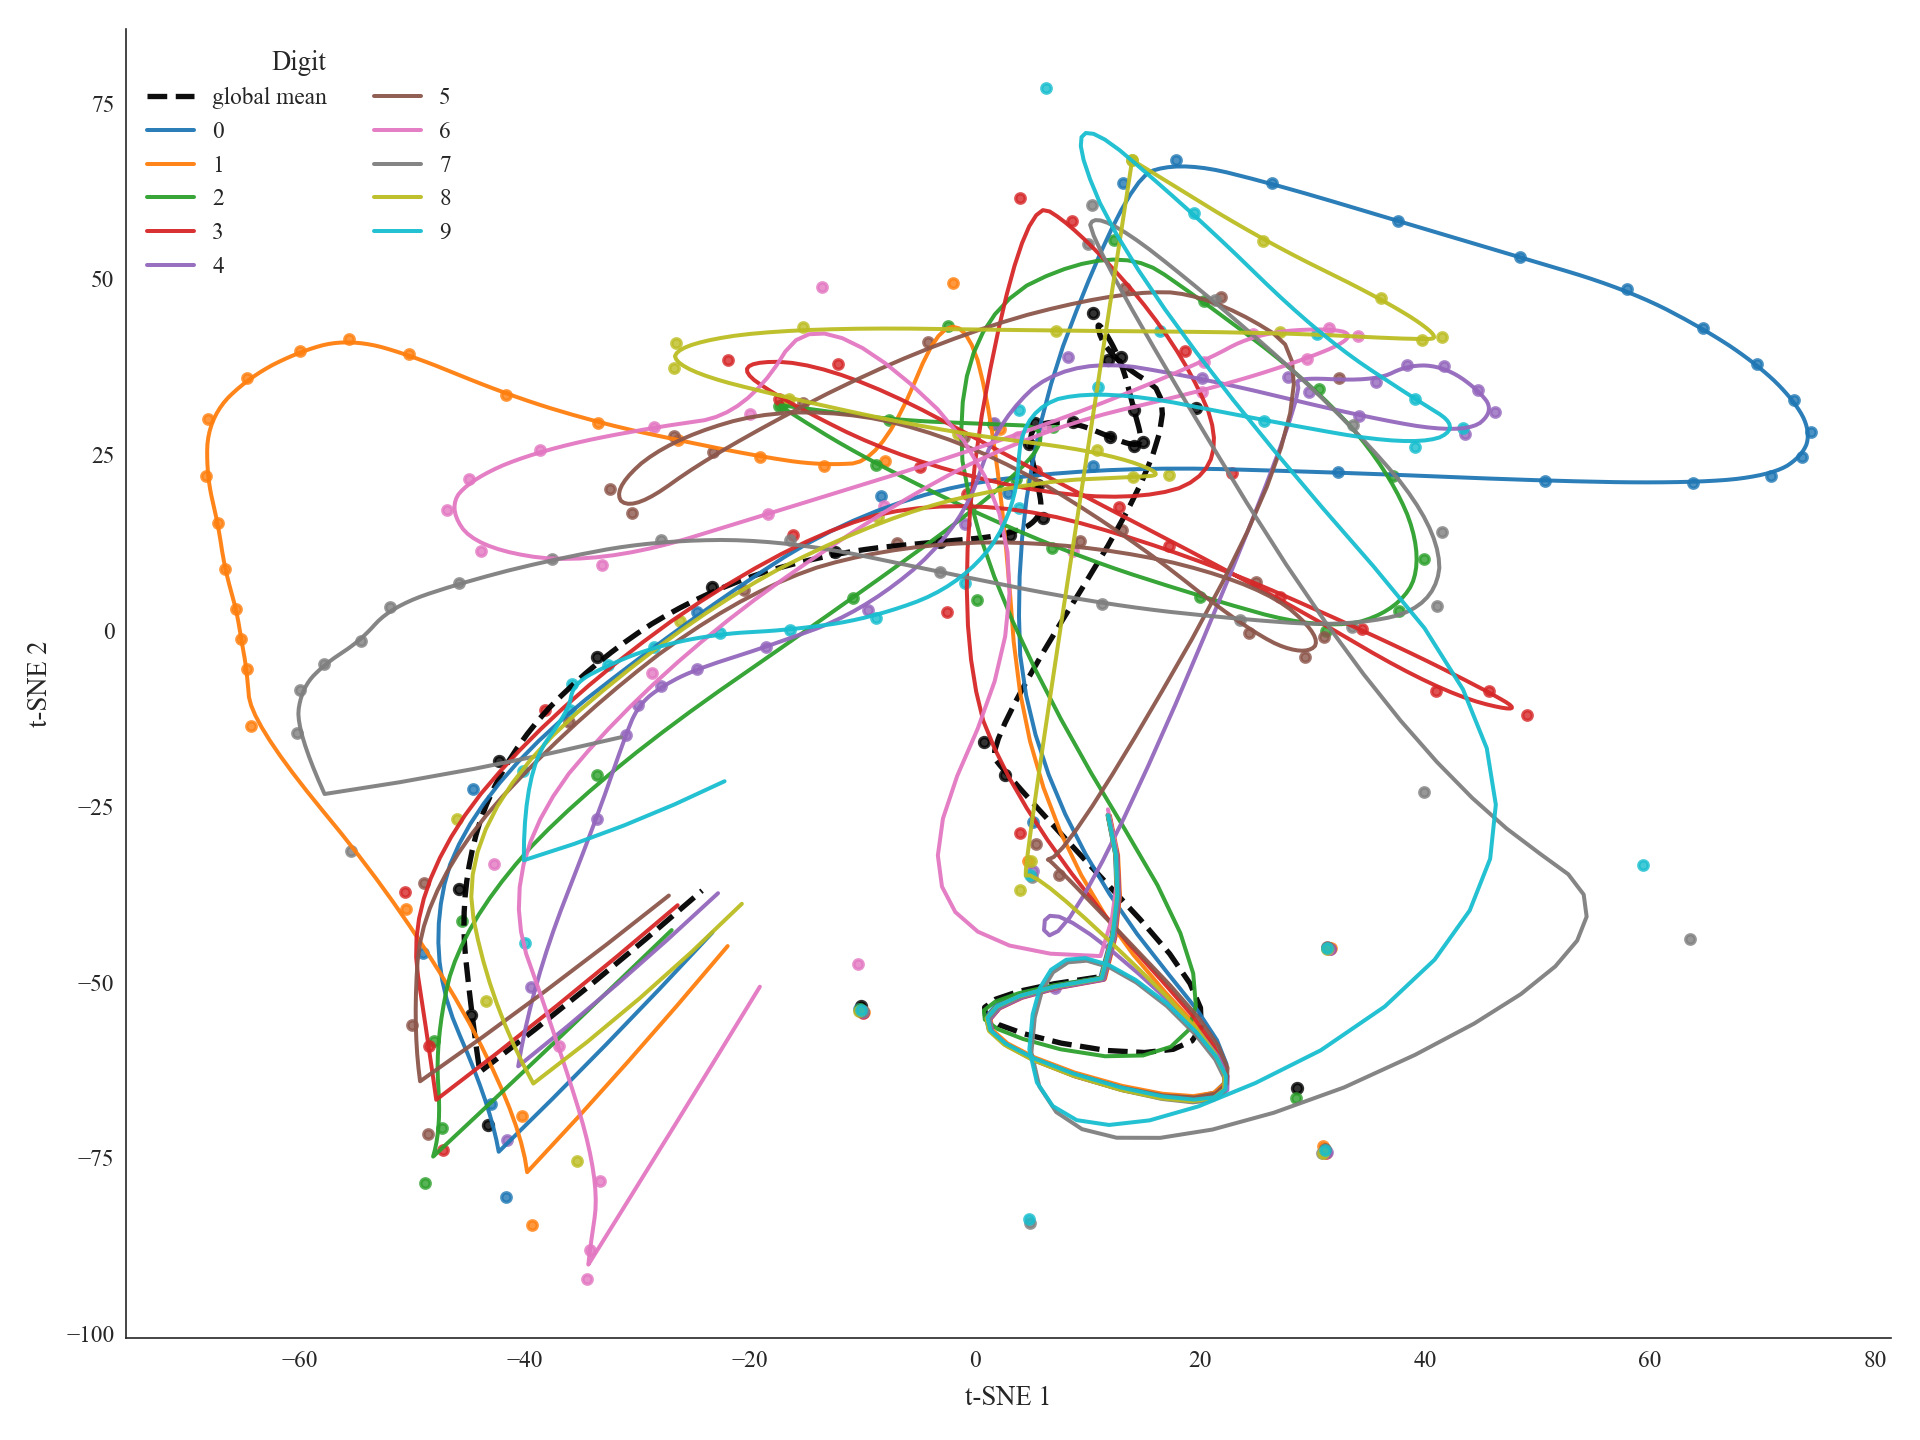
\includegraphics[width=0.49\linewidth]{bp_rnn_mnist_rows/sequence_latent_tsne_mean_paths.png}
  \caption{Smoothed mean trajectories in t-SNE space: a global mean path across all samples and a class-mean path per digit. \textbf{Left:} TeReL. \textbf{Right:} BP.}
  \label{fig:mnist_rows_tsne_mean_paths}
\end{figure}
\FloatBarrier

\begin{figure}[!ht]
  \centering
  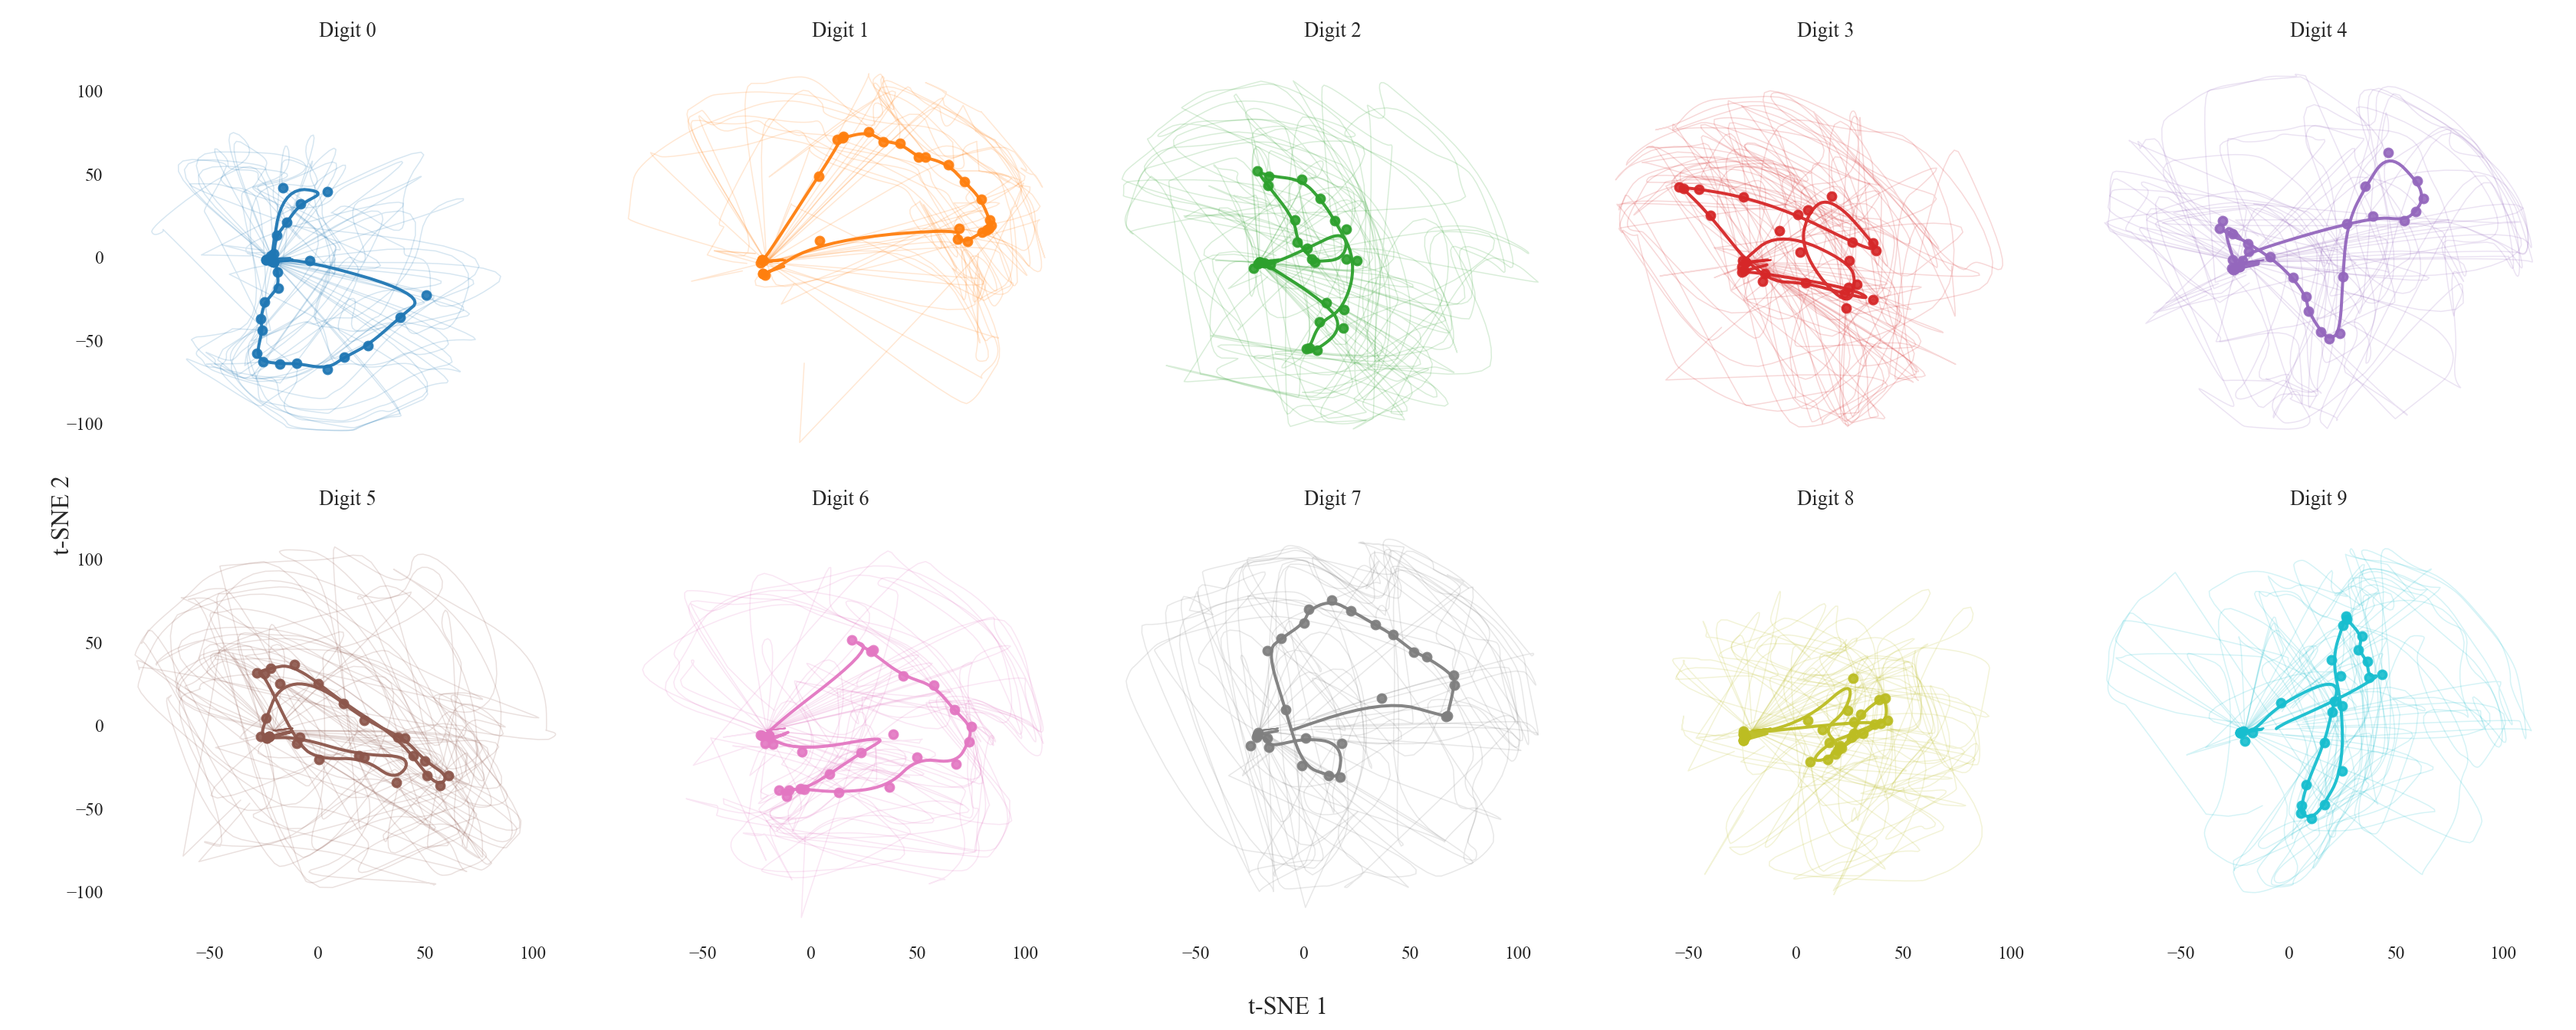
\includegraphics[width=0.49\linewidth]{terel_rnn_20ep/sequence_latent_tsne_per_digit_paths.png}
  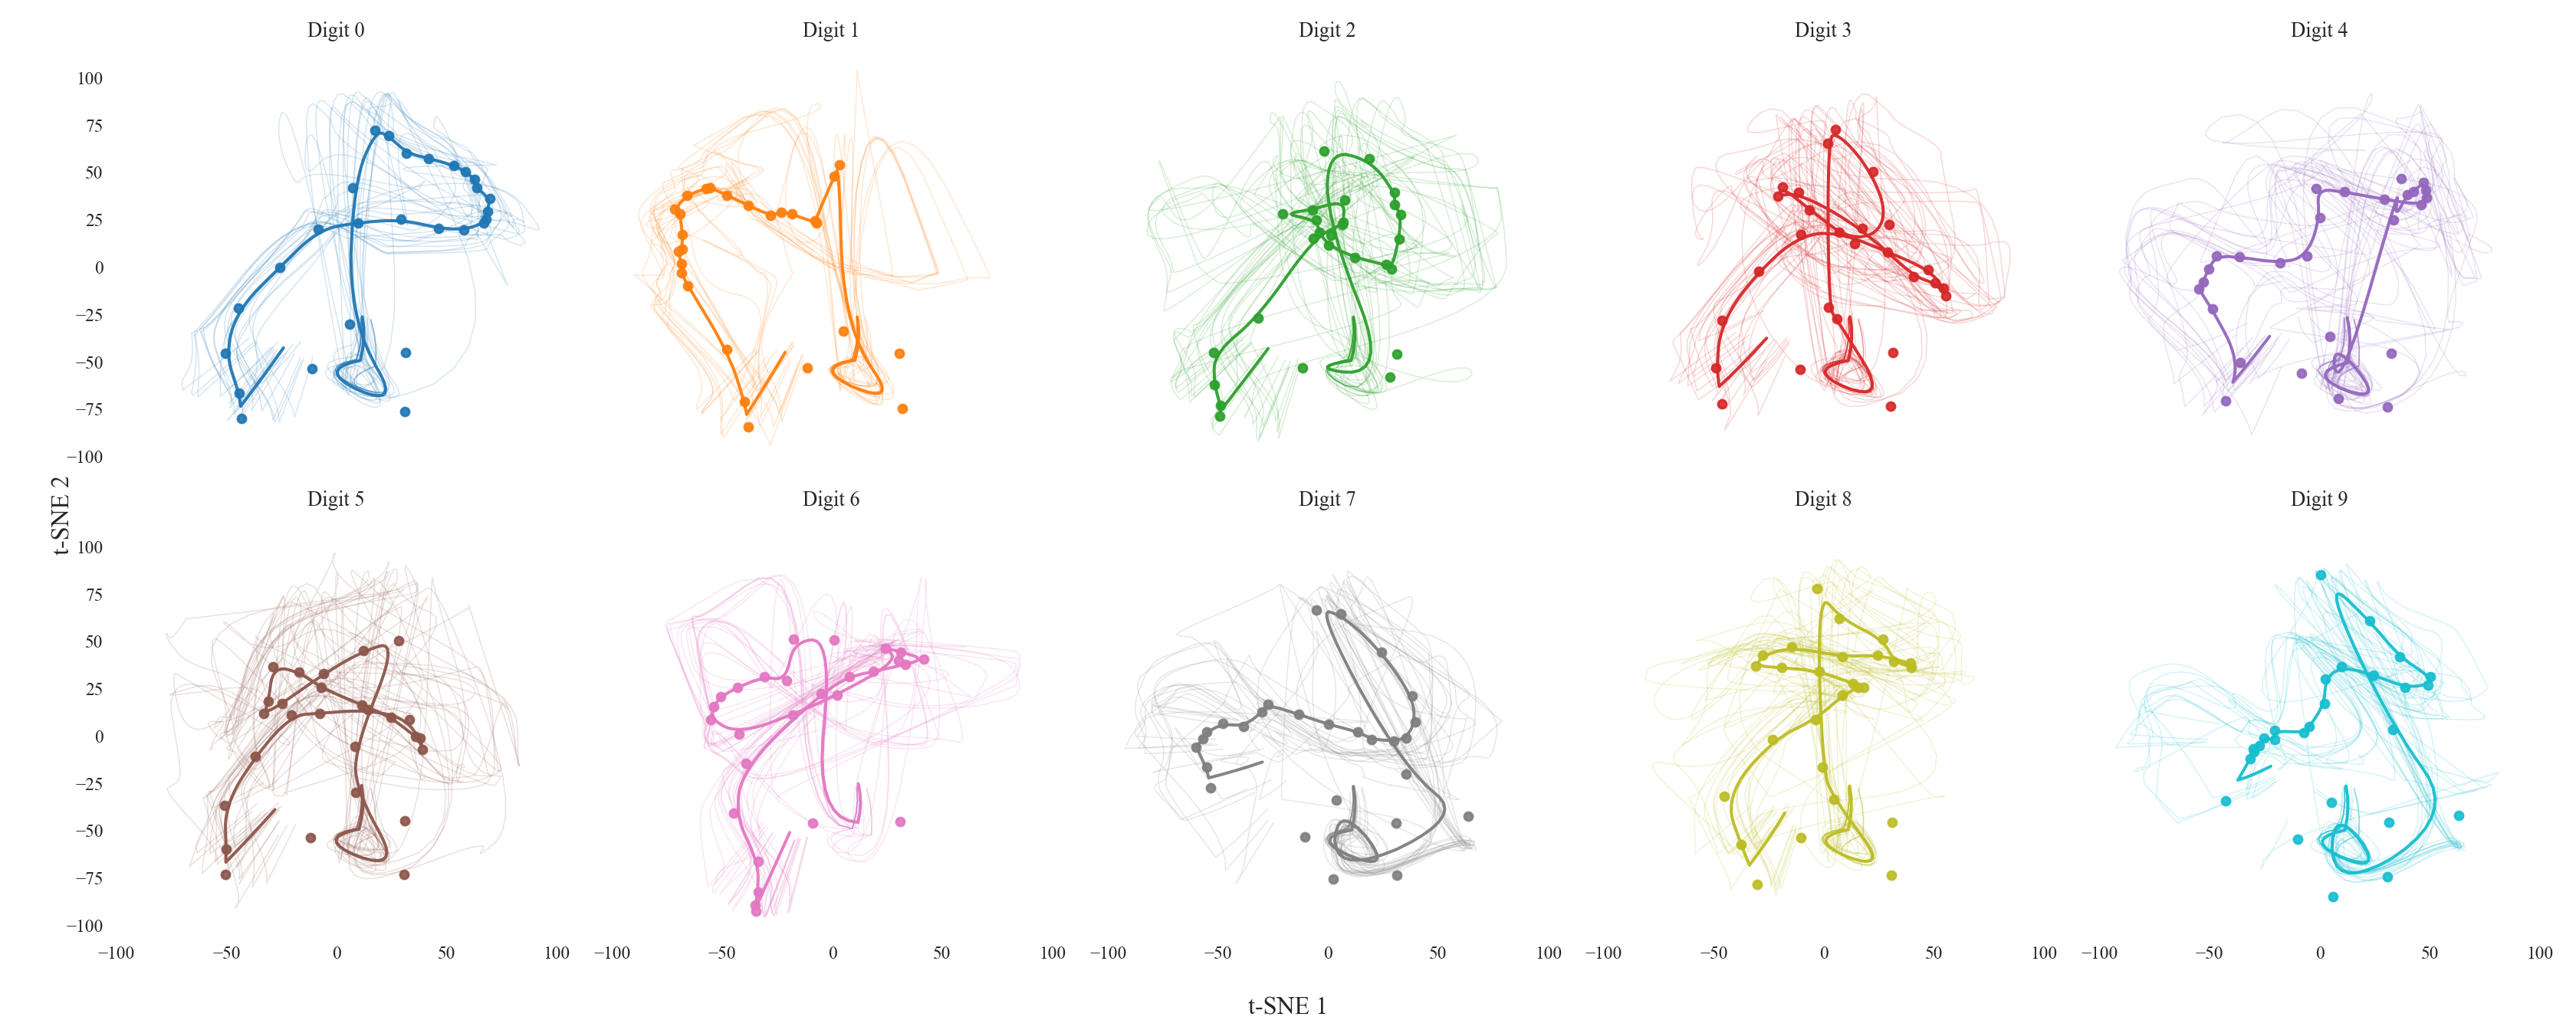
\includegraphics[width=0.49\linewidth]{bp_rnn_mnist_rows/sequence_latent_tsne_per_digit_paths.png}
  \caption{Per-digit trajectory panels in t-SNE space. Each panel shows smoothed sample paths for one digit together with the digit mean path and timestep markers. \textbf{Left:} TeReL. \textbf{Right:} BP.}
  \label{fig:mnist_rows_tsne_per_digit_paths}
\end{figure}
\FloatBarrier

\noindent In this space, both models learn digit-specific progression paths with partial class separability, suggesting a learned row-progression manifold. Qualitatively, TeReL shows particularly clear per-digit structure for digits 0, 1, and 9, while the backpropagation baseline shows this most strongly for digits 2, 4, and 6. While TeReL mean trajectories are more identifiable, backpropagation produces more coherent hidden-state progressions.

\subsection{Architecture details and the role of preprocessing}
Our architecture consists of a preprocessor, a recurrent aggregator, and a linear prediction head. In the TeReL model, we impose the constraint that no backpropagation, including backpropagation through time (BPTT), is performed, preserving an online-compatible update rule.

The model is split into (i) a per-timestep preprocessor that maps the raw row $x_t$ to features $y_t$, (ii) a recurrent aggregator that fuses $(y_t, h_{t-1})$ into a new state $h_t$, and (iii) a linear head that predicts the next row $x_{t+1}$ from $h_t$. In our TeReL sequence model, both the preprocessor and the recurrent aggregator are trained using the TeReL objective, while the linear head is trained for the next-row prediction task.

In our experiments, using a standard RNN-style aggregator directly on raw rows without a preprocessor did not yield meaningful performance. We attribute this to a distribution mismatch between the raw input rows and the evolving hidden state, which makes direct fusion of $(x_t, h_{t-1})$ brittle. Introducing a preprocessor trained with a TeReL objective alleviates this mismatch, since both inputs are represented by a vector optimized under the TeReL-objective.


\section{Limitations and future work}
\FloatBarrier

\subsection{Limitations}
\begin{itemize}
    \item Experiments are limited to MNIST and synthetic temporal orderings. 
    \item Optimizer sensitivity: with the lateral layer in place, TeReL favors adaptive optimizers that consider second moment. Further work is required to reduce optimizer sensitivity or to develop lateral updates that are robust under SGD.
\end{itemize}

\subsection{Future work}

Research directions building on this work include:
\begin{itemize}
    \item Implement a truly online model that uses TeReL.
    \item Measure TeReL performance for sequences of real data or alternative orderings. Explore synthetic sequence ordering as a way to 
    prioritize certain features.
    \item Scale evaluation to natural video and to larger image benchmarks with matched compute budgets.
    \item Examine TeReL for longer autoregressive generation through RNNs. 
    \item Explore alternatives to the lateral layer that reduce optimizer sensitivity while retaining covariance control.
\end{itemize}

\section{Conclusion}

We presented Temporal Regularized Learning, an approach that adapts variance, invariance, and covariance regularizers to neuron-level temporal losses. TeReL yields competitive MNIST performance under controlled temporal orderings and learns highly class-separable representations with rich first-layer receptive fields. Beyond feedforward encoders, we also demonstrated a scoped recurrent setting on MNIST-Rows next-row prediction under a locality constraint, highlighting that TeReL-style objectives can support sequence models without backpropagation through time. TeReL emphasizes locality and streaming compatibility and therefore maps naturally to constrained hardware targets, while connecting regularized self-supervised learning to classical trace-based ideas such as Slow Feature Analysis. Reproducibility and open-code details are provided in the appendix.

\bibliographystyle{unsrt}  
\bibliography{references}  

\appendix

\section{Appendix}

\subsection{Proof details for locality and online implementation}\label{app:locality-proof}
This appendix provides derivation details supporting Proposition~\ref{thm:vicreg-local}. We make explicit (i) the mapping from VICReg invariance to TeReL temporal coherence under a temporal-coherence assumption for choosing positive pairs, and (ii) the local/online state required to implement each term.

\paragraph{Setup and notation.}
Let a layer produce activations $z_t \in \mathbb{R}^D$ at time step $t$, with components $z_{t,j}$. Let each neuron maintain a running mean $m_j$ and running variance estimate $v_j$ (e.g., exponential moving averages), and store the previous activation $p_j=z_{t-1,j}$. Let $\phi$ denote a generic activation function with derivative $\phi'(a)$, where $a$ denotes the pre-activation.

\paragraph{VICReg invariance $\rightarrow$ TeReL temporal coherence.}
VICReg uses an invariance term between paired representations. When inputs are a temporally coherent stream, we can choose the positive for time step $t$ as the previous sample, which corresponds to setting $z_{\mathrm{pos}}=z_{t-1}$. This turns the invariance loss into a temporal-coherence loss
\begin{equation}
L_{S,j} = (z_{t,j}-z_{t-1,j})^2.
\end{equation}
This term is temporally local because it depends only on the current and previous activations.

\paragraph{Variance term is online with bounded state.}
Any variance-maintenance term that depends on deviations from a running mean, e.g. $(z_{t,j}-m_j)^2$, can be implemented online provided $(m_j,v_j)$ are updated incrementally. In TeReL, this is realized with leaky integrators (exponential moving averages), which require only a constant number of scalars per neuron.

\paragraph{Decorrelation term via a lateral mapping (and shifted approximation).}
Decorrelation/whitening-type penalties depend on multi-unit statistics. In TeReL, the required decorrelation signal is provided by a lateral mapping $\mathrm{lat}(\cdot)$ operating on the current (mean-centered) activity vector. When the input to $\mathrm{lat}$ is detached, the learning signal for the main network remains local in the sense that gradients do not backpropagate through other layers. A one-step shift that replaces the current lateral signal by the previous-step signal yields a temporally fully local update as summarized in Proposition~\ref{prop:shifted-lateral-method}.

\subsection{Proof details for the fourfold weighted-sum gradient}\label{app:fourfold-proof}
This appendix provides an algebraic derivation of Proposition~\ref{thm:fourfold-sum}.

\paragraph{Assumed scalar per-neuron loss.}
Let a neuron have pre-activation $a$, activation $z=\phi(a)$, previous activation $p$, and running mean $m$. Consider a per-neuron loss of the form
\begin{equation}
L = \lambda_S (z-p)^2 + \lambda_V (z-m)^2 + \lambda_C\, z\, \mathrm{lat}(\mathrm{detach}(z-m)).
\end{equation}
The lateral input is detached so that $\mathrm{lat}(\cdot)$ is treated as constant w.r.t. the main-network gradient.

\paragraph{Derivative w.r.t. activation.}
Differentiating w.r.t. $z$ yields
\begin{equation}
\frac{\partial L}{\partial z}
= 2\lambda_S(z-p) + 2\lambda_V(z-m) + \lambda_C\,\mathrm{lat}(z),
\end{equation}
where we abbreviate $\mathrm{lat}(z)$ for the lateral output evaluated on the (detached) mean-centered activity.

\paragraph{Per-weight gradient factorization.}
For a synapse with input $x$ into pre-activation $a$, we have $\frac{\partial a}{\partial w}=x$ and $\frac{\partial z}{\partial a}=\phi'(a)$, so
\begin{equation}
\frac{\partial L}{\partial w}
= \frac{\partial L}{\partial z}\frac{\partial z}{\partial a}\frac{\partial a}{\partial w}
= x\,\phi'(a)\Big(2(\lambda_S+\lambda_V)z -2\lambda_S p -2\lambda_V m + \lambda_C\,\mathrm{lat}(z)\Big),
\end{equation}
which is the fourfold weighted-sum form stated in Proposition~\ref{thm:fourfold-sum}.

% Trace learning vs. TeReL temporal-coherence: detailed algebra (moved from main text)
\section{Trace learning vs.\ TeReL temporal-coherence: algebraic comparison}
\label{app:trace-terel-derivation}

This appendix section provides the detailed derivation supporting Proposition~\ref{prop:trace-incompatibility}.

\paragraph{TeReL temporal coherence.}
Starting from the temporal-coherence term (for neuron $j$ at time $t$)
\begin{equation}
L_{S,t,j} = (z_{t,j}-z_{t-1,j})^2,
\end{equation}
the gradient contribution for a weight $w_{k j}$ into neuron $j$ is
\begin{align}
\Delta w_{k j} &\propto -\frac{\partial L_{S,t,j}}{\partial w_{k j}}
= -\frac{\partial L_{S,t,j}}{\partial z_{t,j}}
\frac{\partial z_{t,j}}{\partial a_{t,j}}
\frac{\partial a_{t,j}}{\partial w_{k j}} \\
&= 2(z_{t-1,j}-z_{t,j}) \, \phi'(a_{t,j}) \, x_k,
\end{align}
where $a_{t,j}$ is the pre-activation and $z_{t,j}=\phi(a_{t,j})$.

\paragraph{Trace learning.}
In F\"oldi\'ak-style trace learning, the update is of the form
\begin{equation}
\Delta w_{k j} = \alpha\,\bar z_{t,j}\,(x_k - w_{k j}),
\end{equation}
with an activation trace $\bar z$ maintained as an exponential moving average
\begin{equation}
\bar z_{t,j} \leftarrow \beta\,\bar z_{t-1,j} + (1-\beta)\,z_{t,j}, \qquad \beta\in(0,1).
\end{equation}
Ignoring the weight-decay term (the $-\,\alpha\,\bar z\,w$ component), this yields an update proportional to
\begin{equation}
\Delta w_{k j} \propto x_k\,(\beta\,\bar z_{t-1,j} + (1-\beta)\,z_{t,j}).
\end{equation}

\paragraph{Why they cannot be made identical by choosing $\beta$.}
TeReL's temporal-coherence update is proportional to $x_k\,(z_{t-1,j}-z_{t,j})$ (up to $\phi'(a)$), i.e.\ it requires coefficients $(+1,-1)$ on $(z_{t-1,j},z_{t,j})$. A single-parameter EMA trace produces coefficients $(\beta,\,1-\beta)$ on $(\bar z_{t-1,j},z_{t,j})$, and even if one informally identifies $\bar z_{t-1,j}$ with $z_{t-1,j}$, matching $(+1,-1)$ would require $\beta=1$ and $1-\beta=-1$ simultaneously, which is impossible.


\subsection{Reproducibility and open code}

All of the runs are contained in the publicly available repository. The commit at the time of running the experiments was 25908634afa795840b0026d8481fa69338e857ec for backpropagation and b39b73fac94e984f089820bec7a421499bcd6c0d for the TeReL and TeReL-S setups. 
Different runs are configured by modifying the unified configuration class with functions at runtime. The setup is configured and the run function called in \texttt{train.py}. Depending on the configuration, we use multiple modifying functions.
The configuration is set up for a TeReL-S run by default. These functions map to the setups in the following way:

\begin{table}[h!]
 \caption{Configuration Functions for Different Experimental Setups}
  \centering
  \begin{tabular}{ll}
    \toprule
    \textbf{Function} & \textbf{Description} \\
    \midrule
    \texttt{long\_training} & 60 epoch long training used for the experiments \\
    \texttt{standard\_setup} & TeReL setup \\
    \texttt{eqprop\_scale\_network} & Network layout for comparison to Equilibrium Propagation, \\ & i.e. 3 hidden layers with 500 units respectively. \\
    \texttt{ff\_scale\_network} & Network layout for comparison to the Forward Forward \\ & procedure, i.e. 4 hidden layers with 2000 units respectively. \\
    \texttt{aug\_and\_rbn\_setup} & Augmentations and batchnorm activated. \\
    \bottomrule
  \end{tabular}
  \label{tab:config_functions}
\end{table}

Backpropagation was tested with a separate script, included in the \texttt{comparison} folder. We ran the experiments on seeds 42 to 46, inclusive. We tuned the learning rate of backpropagation and used the smallest model architecture for tuning the TeReL setups.

% Experimental setup details moved from the main text to keep Section 4 slim.
\section{Experimental setup details}
\label{app:exp-setup}

\noindent Table~\ref{tab:setup} summarizes the shared experimental settings used for the MNIST results reported in the main text.

\begin{table}[h]

\caption{Experimental Setup}
\centering
\begin{tabular}{lll}
\toprule
\textbf{Parameter} & \textbf{Applies to} & \textbf{Value} \\
\midrule
Epochs & All & 60 \\
Activation Function & All & ReLU \\
Seeds & TeReL(-S), backprop & 42 to 46 \\
Optimizer & TeReL(-S), backprop & Adam \\
Batch size & TeReL(-S), Backprop & 64 \\
Neuron statistics & TeReL(-S) & In-Batch detached \\
Chunk size & TeReL(-S) & 16 \\
Covariance matrix implementation & TeReL(-S) & Lateral mapping \\
\bottomrule
\end{tabular}
\label{tab:setup}\end{table}
\FloatBarrier



% Hyperparameter guidance moved from the main experiments section.
\section{Guidance for choosing hyperparameters}
\label{app:hyperparam-guidance}

This section summarizes practical guidance for selecting TeReL hyperparameters based on our ablations.

\paragraph{Choice of loss coefficients and learning rate.}
In the general case, $\lambda_S+\lambda_C<\lambda_V$ prevents collapse, since both similarity and covariance penalize the magnitude of the activation.
The main move in terms of parameter tuning is to change the variance loss for some situations:
\begin{itemize}
    \item If we detach the previous activation (as we do in the TeReL-S setup), experimentation has shown that doubling the variance coefficient is beneficial.
    \item If we use batch normalization, we can quadruple the learning rate and halve the variance loss coefficient.
    \item And if we use SGD, we double the variance loss coefficient.
\end{itemize}


% Appendix details for MNIST-Rows sequence prediction experiments
\subsection{MNIST-Rows sequence prediction: additional details}\label{app:rnn-details}

This appendix complements Section~\ref{sec:mnist_rows_rnn} with additional qualitative rollout plots.


\paragraph{Autoregressive rollouts.}
We additionally include multi-step autoregressive row-completion rollouts to visually show next-element predictions of the two models. For each sample, the model is conditioned on 8, 16, or 24 of the image's first rows and predicts the next 4 rows; the remaining rows are shown as ground truth. The first red marker indicates the context-to-generation boundary, and the second red marker indicates the generation-to-ground-truth boundary. These rollouts are included for visual inspection, and long-horizon stability is not optimized in this study and rollout quality is not treated as a primary evaluation metric.


\begin{figure}[!ht]
  \centering
  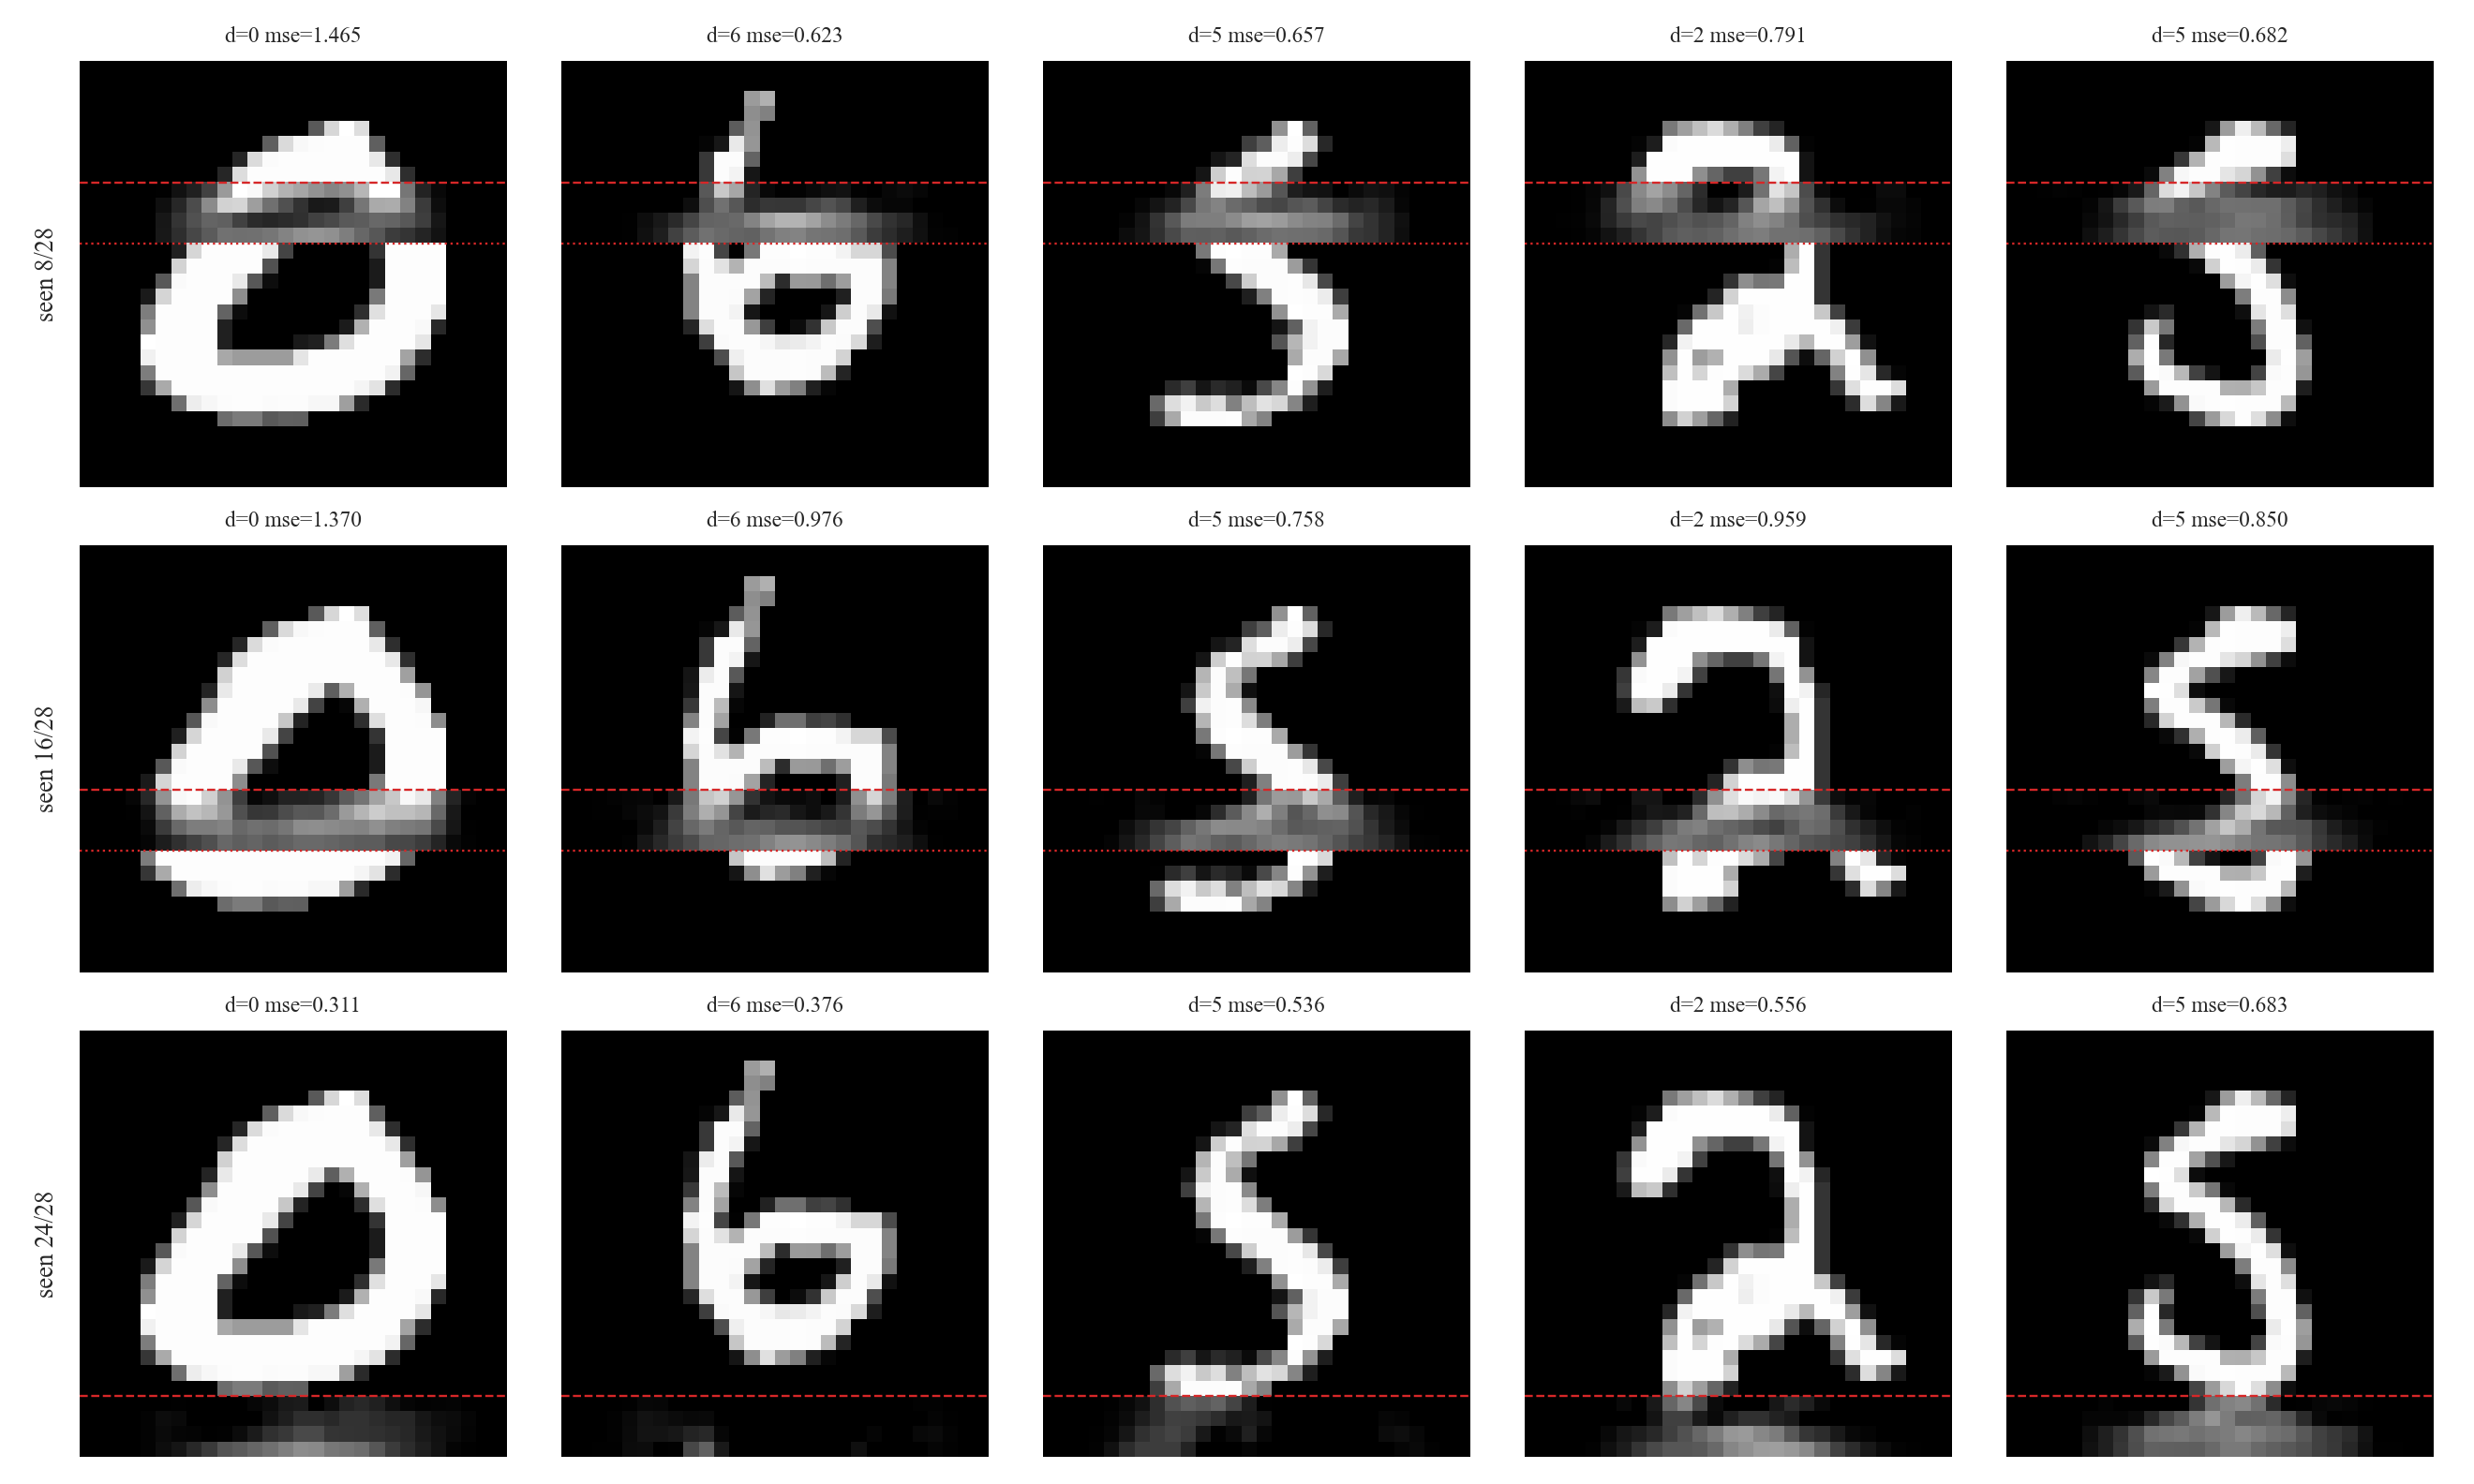
\includegraphics[width=0.49\linewidth]{terel_autoregressive_rows4_ctx_2_4_6of7.png}
  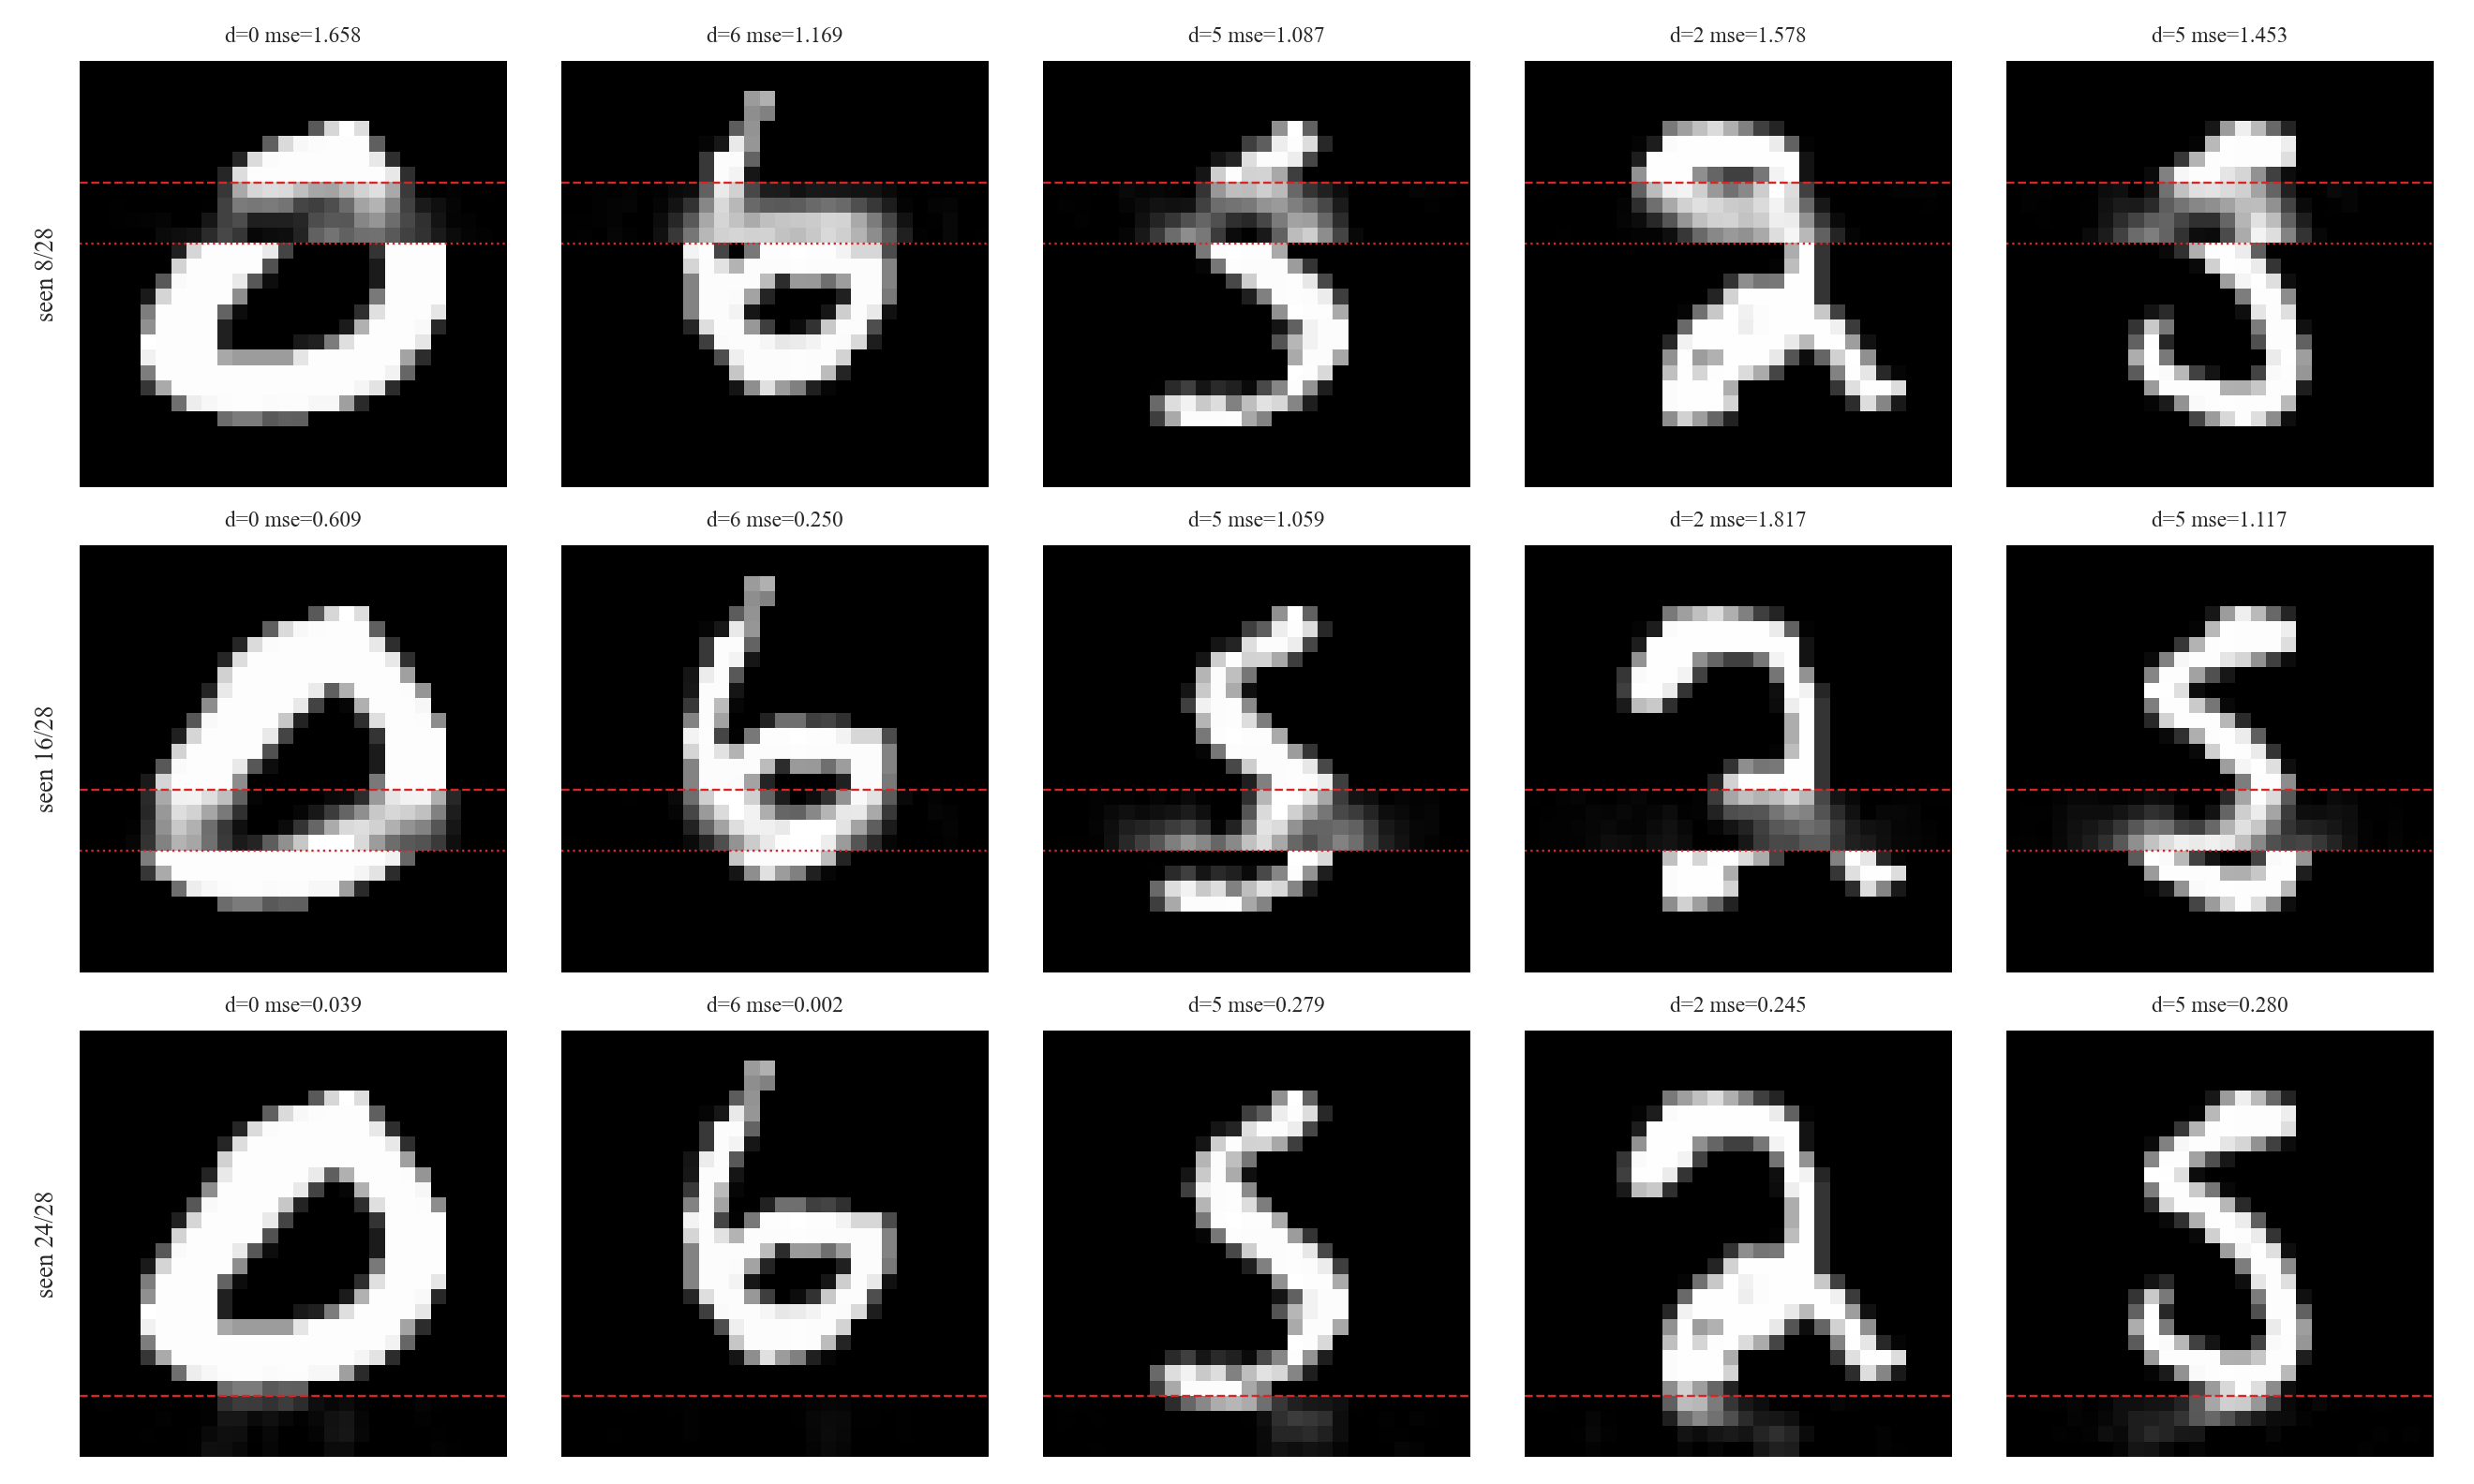
\includegraphics[width=0.49\linewidth]{bp_autoregressive_rows4_ctx_2_4_6of7.png}
  \caption{Autoregressive row completion on MNIST-Rows (left: TeReL, right: BP).}
  \label{fig:mnist_rows_rollout_rows4_ctx}
\end{figure}
\FloatBarrier

\noindent The TeReL setup used for these rollouts was trained concurrently. The exact repository state at the point of generation is recorded in the repository README.


% Ablation result tables moved from the main text.
\section{Ablation results and run specifications}
\label{app:ablation-results}

This section reports additional ablation metrics and summarizes the configuration changes for each run (see the repository artifacts \texttt{terel\_ablation\_results.csv} and \texttt{terel\_ablation\_run\_specs.md}).

\begin{table}[h]
\caption{Ablation results}
\centering
\resizebox{\linewidth}{!}{%
\begin{tabular}{lrr}
\toprule
\textbf{Description} & \textbf{Validation accuracy} & \textbf{Validation error} \\
\midrule
TeReL reference setup & 0.9691 & 0.0309 \\
Head uses only last hidden layer & 0.9633 & 0.0367 \\
Trace activation enabled & 0.9542 & 0.0458 \\
One-step shifted lateral signal & 0.9165 & 0.0835 \\
Trace with faster decay & 0.9711 & 0.0289 \\
Lateral shift + shifted covariance target & 0.9518 & 0.0482 \\
Trace fast + lateral shift + fast covariance & 0.9336 & 0.0664 \\
Trace + lateral shift + last-layer head & 0.9120 & 0.0880 \\
TeReL-S reference setup & 0.9658 & 0.0342 \\
Shift + shifted covariance target + last-layer head & 0.9289 & 0.0711 \\
Trace fast + shift + shifted covariance target + last-layer head & 0.9204 & 0.0796 \\
\bottomrule

\end{tabular}
}
\label{tab:ablation-results}
\end{table}

% Naming legend removed (table uses descriptive labels; run-spec details remain in repository artifacts).


Preliminary versions are contained in the \texttt{previous\_versions} folder. These versions form a path from VICReg to TeReL: each script has changes relative to its predecessor, which are briefly explained in the README file of the folder. We can see that a shifted lateral signal can yield nontrivial performance in this setup. 

\subsection{Runs}
\paragraph{Backprop runs by seed (validation accuracy in \%)}
\begin{table}[h!]
\centering
\begin{tabular}{llllllllll}
\toprule
\textbf{Hidden Layers} & \textbf{Aug \& BN} & \textbf{42} & \textbf{43} & \textbf{44} & \textbf{45} & \textbf{46} & \textbf{Mean} & \textbf{Error} \\
\midrule
512, 256           & Y & 98.77 & 98.94 & 98.91 & 98.85 & 98.98 & 98.89 & 1.11  \\
                   & N & 97.70 & 97.93 & 98.17 & 98.14 & 97.97 & 97.98 & 2.02  \\
500 thrice         & N & 98.13 & 97.81 & 98.06 & 98.07 & 97.87 & 97.99 & 2.01  \\
4 layers 2000 each & N & 98.12 & 98.17 & 97.99 & 98.29 & 98.04 & 98.12 & 1.88  \\
\bottomrule
\end{tabular}
\end{table}

\paragraph{TeReL runs by seed}
\begin{table}[h!]
\centering
\begin{tabular}{llllllllll}
\toprule
\textbf{Hidden Layers} & \textbf{Aug \& BN} & \textbf{42} & \textbf{43} & \textbf{44} & \textbf{45} & \textbf{46} & \textbf{Mean} & \textbf{Error} \\
\midrule
512,256            & Y & 98.47 & 98.23 & 98.28 & 98.03 & 98.19 & 98.24 & 1.76  \\
                   & N & 97.01 & 96.85 & 97.00 & 97.07 & 97.01 & 96.99 & 3.01  \\
500 thrice         & N & 96.69 & 96.76 & 96.82 & 96.68 & 96.87 & 96.75 & 3.25  \\
4 layers 2000 each & N & 98.10 & 98.13 & 97.98 & 97.85 & 97.89 & 97.99 & 2.01  \\
\bottomrule
\end{tabular}
\end{table}

\paragraph{TeReL-S runs by seed}
\begin{table}[h!]
\centering
\begin{tabular}{llllllllll}
\toprule
\textbf{Hidden Layers} & \textbf{Aug \& BN} & \textbf{42} & \textbf{43} & \textbf{44} & \textbf{45} & \textbf{46} & \textbf{Mean} & \textbf{Error} \\
\midrule
512,256            & Y & 97.84 & 97.58 & 97.61 & 97.84 & 97.72 & 97.72 & 2.28  \\
                   & N & 96.53 & 96.30 & 96.51 & 96.42 & 96.51 & 96.45 & 3.55  \\
500 thrice         & N & 96.54 & 96.42 & 96.48 & 96.50 & 96.19 & 96.43 & 3.57  \\
4 layers 2000 each & N & 97.51 & 97.65 & 97.72 & 97.58 & 97.68 & 97.63 & 2.37  \\
\bottomrule
\end{tabular}
\end{table}

\paragraph{Parameter counts by model layout and setup:}
\begin{table}[h!]
\centering
\begin{tabular}{llll}
\toprule
\textbf{Setup} & \textbf{Hidden Layers} & \textbf{Inference Params} & \textbf{Auxiliary Params} \\
\midrule
Backprop, FF, EqProp & 512, 256      & 535K                 & -                    \\
                     & 500 thrice    & 897K                 & -                    \\
                     & 4 x 2000      & 13.59M               & -                    \\
TeReL, TeReL-S           & 512, 256      & 540K                 & 328K                 \\
                     & 3 x 500       & 907K                 & 750K                 \\
                     & 4 x 2000      & 13.65M               & 8M                   \\
\bottomrule
\end{tabular}
\end{table}

Auxiliary parameters are the lateral mappings that are optimized to match the covariance matrix. We consider sparsity when reporting them. We enforce sparsity by randomly selecting entries of the target covariance matrix that are consistently zeroed out. The largest model layout has a sparsity of 50\%, others have a sparsity of 0\%.

\ifdefined\HCode
  \ifvmode\IgnorePar\fi\EndP
  \HCode{</main>}\ShowPar
\fi


\end{document}
